%%%%(c)
%%%%(c)  This file is a portion of the source for the textbook
%%%%(c)
%%%%(c)    Abstract Algebra: Theory and Applications
%%%%(c)    Copyright 1997 by Thomas W. Judson
%%%%(c)
%%%%(c)  See the file COPYING.txt for copying conditions
%%%%(c)
%%%%(c)
\chap{Error-Detecting and Correcting Codes\quad
\sectionvideohref{EOKgMvWuBpc&list=PL2uooHqQ6T7PW5na4EX8rQX2WvBBdM8Qo&index=39}}{chap:ErrorAndCorrectionCode}
 
In Chapter~\ref{crypt} we looked at  cryptography, which is concerned with the encoding of  information to make it secret. But coding is used for other purposes as well.  When data is transmitted, it is often subject to processes which may corrupt the data and produce transmission errors. This situation
arises in many areas of communications, including radio, telephone, television, computer communications, and even compact disc player technology. In order to guarantee accurate communication, the data must be encoded (before transmission) and decoded (after transmission) so that transmission errors can be detected and, if possible, corrected. As you may imagine,  some of the world's leading high-tech companies are heavily involved in this area--and breakthroughs can mean big bucks for the discoverers!
\medskip

\noindent
\underline{\bf Prerequisites}: In this chapter we will make extensive use of the group $\mathbb{Z}^{n}_{2}$, which is the direct product of $n$ copies of $\mathbb{Z}_{2}$ (direct products were introduced in Section~\ref{sec:isomorph_section_2}.  
%Section~\ref{sec:MaximumLikelihood} on maximum-likelihood decoding uses some probability theory--this section is independent of the rest of the chapter, and may be omitted if desired. 
The discussion of linear block codes (Section~\ref{sec:algcodes:BlockCodes} and following) uses concepts from linear algebra such as matrix, vector, and matrix multiplication. Section \ref{sec:efficientDecoding} uses some basic ideas about cosets, which were introduced in  Chapter~\ref{cosets}.  
\bigskip

Thanks to Tom Judson for material used in this chapter.
  
 
\section{Definitions and basic properties}
\label{sec:ErrorAndCorrectionCode:Definitions}
  
Let's examine a simple model of a communications system for
transmitting and receiving coded messages (Figure~\ref{encoding}).  
\begin{figure}[htbp]
\begin{center}
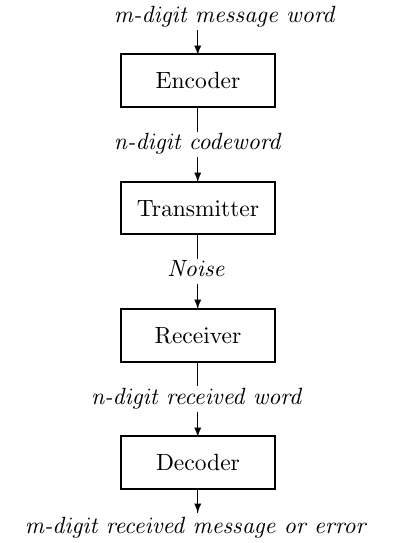
\includegraphics{images/simpleCommModel.png}
\end{center}
\caption{Encoding and decoding messages\label{encoding}}
\end{figure}
Uncoded messages consist of a sequence of symbols, such as letters or characters. Now when computers do calculations they can't understand letters: they can only understand sequences consisting of 0's and 1's (0 and 1 are referred to as binary digits or \term{bits}).  So before coding, individual symbols are  re-expressed as sequences of binary bits, and then these bits are strung together to form a single sequence of bits which expresses the message content.  This sequence is divided up into chunks (or tuples) of $m$ bits apiece: these binary $m$-tuples
are referred to as \term{message words}. Message words are
then encoded into \term{codewords}\index{Codeword} of $n$ bits apiece by a device
called an \term{encoder}\index{Encoder}. These codewords are transmitted over a channel and received by a receiver.
Random noise in this transmission process causes some of the bits to be corrupted: and we say that 
 an \term{error} \index{Error}occurs every time a bit is changed from 0 to 1 or vice-versa due to transmission noise.The \term{decoder} converts
each received $n$-tuple into a message word or
gives an error message for that $n$-tuple. If the recieved codeword was not corrupted by random noise during transmission,
then the decoded message word will agree with the original message word. For received words that are not codewords, the decoding scheme will
give an error indication, or (in the case of error-correcting codes) will try
to correct the error and reconstruct the original message word. The  goal is
to transmit error-free messages as cheaply and quickly as possible.

\begin{exercise}{}
Why is the following encoding scheme not acceptable?
\[
\begin{array}{lcccccccccc}
\hline
\mbox{Information:} & 0 & 1 & 2 & 3 & 4 & 5 & 6 & 7 & 8 &
\\ \hline
\mbox{Codeword:} & 000 & 001 & 010 & 011 & 101 & 110
& 111 & 000 & 001 \\ \hline
\end{array}
\]
 \end{exercise} 
 
\begin{example}{evenParity}
\term{Even parity}\index{Even parity!coding scheme} is a  commonly  used coding scheme, which (as we shall see) can be generalized to form powerful and versatile codes. Computers use the ASCII (American
Standard Code for Information Interchange) coding system to encode the letters and special characters that appear on your keyboard (these may be considered as the "message words", according to the above terminology). There are 128 of these characters, so it is possible to represent them using 7 bits (since  $128 = 2^7$).   For example, the 7-bit representations for A, B, and C are 
\begin{align*}
\textrm{A} & = 1000001, \\
\textrm{B} & = 1000010, \\
\textrm{C} & =  1000011.
\end{align*}
Although 7 bits are sufficient, the ASCII code uses 8 bits for each charater. A bit is added to the front of the codeword according to the following rule:  if the number of 1's in the seven-bit 
representation is even, then the front bit is 0; otherwise, the front bit is 1. 
According to this rule, the 8-bit codes
for A, B, and C now become 
\begin{align*}
\textrm{A} & = & 01000001, \\
\textrm{B} & = & 01000010, \\
\textrm{C} & = & 11000011.
\end{align*}
Notice that these 8-bit codes all have an \emph{even} number of 1's.

Now suppose an A is sent and a transmission error in the sixth
bit is caused by noise over the communication channel so that 
(01000101) is received. We know an error has occurred since the
received word has an odd number of 1's, and we can now request that the
codeword be transmitted again. When used for error checking, the
leftmost bit is called a \term{parity check bit}\index{Parity!parity check bit}.  
  
Adding a parity check bit allows the detection of all single errors
because changing a single bit either increases or decreases the number
of 1's by one, and in either case the parity has been changed from
even to odd, so the new word is not a codeword. (We could equally well
construct an error detection scheme based on \term{odd parity}\index{Parity!odd}, where the parity check bit is set so that codewords always have an
odd number of 1's.)  
\end{example} 

The even parity system is easy to implement, but has two drawbacks.
First, multiple errors are not detectable. Suppose an A is sent and 
the first and seventh bits are changed from 0 to 1. The received word
is a codeword, but will be decoded into a C instead of an A.
Second, we do not have the ability to correct errors.  If the 8-tuple
(10011000) is received, we know that an error has occurred, but we
have no idea which bit has been changed. We will now investigate a
coding scheme that will not only allow us to detect transmission
errors but will actually correct the errors. 

\begin{example}{bit3}
Suppose that our original message is either a 0 or a 1, and that 0
encodes to (000) and 1 encodes to (111). If only a single
error occurs during transmission, we can detect and correct the
error. For example, if a 101 is received, then the second bit must
have been changed from a 1 to a 0.  The originally transmitted
codeword must have been (111). 	This method will detect and correct 
all single errors. 
 
 
In Table~\ref{algcodes:table0}, we present all possible words that might be received
for the transmitted codewords (000) and (111). Table~\ref{algcodes:table0} also shows 
the number of bits by which each received 3-tuple differs from each
original codeword. 

 
\begin{table}[htb]
\caption{A repetition code\label{algcodes:table0}}{\small
\begin{center}
\begin{tabular}{|lc|cccccccc|}
\hline
& & \multicolumn{8}{|c|}{Received Word}    \\
            &     & 000 & 001 & 010 & 011 & 100 & 101 & 110
& 111 \\ \hline
Transmitted & 000 & 0   & 1   & 1   & 2   & 1   & 2   & 2
& 3 \\
Codeword   & 111 & 3   &  2  & 2   &  1  &  2  &   1 &  1
&  0 \\ \hline
\end{tabular}
\end{center}
}
\end{table}

This triple-repetition method \index{Repetition!encoding}will automatically detect and correct
all single errors, but it's not very efficient (just imagine having to repeat everything you say three times in order to make yourself understood!)  We'll see shortly that there are much better alternatives.
\end{example}

%\subsection{Maximum-Likelihood Decoding\quad
%\sectionvideohref{EOKgMvWuBpc&list=PL2uooHqQ6T7PW5na4EX8rQX2WvBBdM8Qo&index=39}}\label{sec:MaximumLikelihood}
% 
%\begin{quote}
%\emph{This section
%requires a knowledge of probability, It can be
%skipped without loss of continuity.} 
%\end{quote}
%
%The coding scheme presented in Example~\ref{example:algcodes:bit3} is not a complete solution to
%the problem because it does not account for the possibility of
%multiple errors. For example, either a (000) or a (111) could be sent
%and a (001) received. We have no means of deciding from the received
%word whether there was a single error in the third bit or two errors,
%one in the first bit and one in the second.  No matter what coding 
%scheme is used, an incorrect message could
%be received: we could transmit a (000), have errors in all three
%bits, and receive the codeword (111). It is important to make explicit
%assumptions about the likelihood and distribution of transmission
%errors so that, in a particular application, it will be known whether
%a given
%error detection scheme is appropriate. We will assume that
%transmission errors are rare, and, that when they do occur, they occur
%independently in each bit; that is, if $p$ is the probability of an
%error in one bit and $q$ is the probability of an error in a different
%bit, then the probability of errors occurring in both of these bits at
%the same time is $pq$. We will also assume that a received $n$-tuple 
%is
%decoded into a codeword that is closest to it; that is, we assume that
%the receiver uses \term{maximum-likelihood
%decoding}\index{Maximum-likelihood decoding}.
% 
% \begin{figure}[htb]
%\begin{center}
%\setlength{\unitlength}{.1in}
%\begin{picture}(14,9)
%\put(2,2){\vector(1,0){10}}
%\put(2,8){\vector(1,0){10}}
%\put(2,2.5){\vector(2,1){10}}
%\put(2,7.5){\vector(2,-1){10}}
%\put(0.8,7.5){\small 0}
%\put(0.8,1.6){\small 1}
%\put(12.6,7.5){\small 0}
%\put(12.6,1.6){\small 1}
%\put(6.5,8.6){\small $p$}
%\put(6.5,1){\small $p$}
%\put(7.5,6){\small $q$}
%\put(7.5,3.5){\small $q$}
%\end{picture}
%\end{center}
%\caption{Binary symmetric channel}
%\label{channel}
%\end{figure}
% 
%A \term{binary symmetric channel}\index{Binary symmetric channel}
%is a model that consists of a transmitter capable of sending a binary 
%signal, either a 0 or a 1, together with a receiver. Let $p$ be the 
%probability that the signal is correctly
%received. Then $q=1-p$ is the probability of an incorrect reception.
%If a 1 is sent, then the probability that a 1 is received is $p$ and
%the probability that a 0 is received is $q$ (Figure~\ref{channel}).
%The probability that no errors occur during the transmission of a binary
%codeword of length $n$ is $p^{n}$. For example, if $p=0.999$ and a
%message consisting of 10,000 bits is sent, then the probability of a
%perfect transmission is 
%\[
%(0.999)^{10,000} \approx 0.00005.
%\]
% 
% \begin{prop}{}
%If a binary $n$-tuple $(x_{1}, \ldots, x_{n})$ is transmitted across a
%binary symmetric channel with probability $p$ that no error will occur
%in each coordinate, then the probability that there are errors in
%exactly $k$ coordinates~is \index{Error!probability of}
%\[
%\left(
%\begin{array}{c}
%n \\ k
%\end{array}
%\right)
% q^kp^{n-k}.
%\]
%\end{prop}
%  
%\begin{proof}
%Fix $k$ different coordinates. We first compute the probability that
%an error has occurred in this fixed set of coordinates. The
%probability of an error occurring in a particular one of these $k$
%coordinates is $q$; the probability that an error will not occur
%in any of the remaining $n-k$ coordinates is $p$. The
%probability of each of these $n$ independent events is
%$q^{k}p^{n-k}$. The number of possible error patterns with exactly $k$
%errors occurring is equal to 
%\[
%\left(
%\begin{array}{c}
%n \\ k
%\end{array}
%\right)
%= \frac{n!}{k!(n-k)!},
%\]
%the number of combinations of $n$ things taken $k$ at a time. Each of
%these error patterns has probability $q^{k}p^{n-k}$ of occurring;
%hence, the probability of all of these error patterns is
%\[
%\left(
%\begin{array}{c}
%n \\ k
%\end{array}
%\right)
%q^{k}p^{n-k}.
%\]
%\end{proof}
% 
% 
%\begin{example}{}
%Suppose that $p = 0.995$ and a 500-bit message is sent. The
%probability that the message was sent error-free is 
%\[
%p^{n} = (0.995)^{500} \approx 0.082.
%\]
%The probability of exactly one error occurring is
%\[
%\left(
%\begin{array}{c}
%n \\ 1
%\end{array}
%\right)
%qp^{n-1}= 500(0.005)(0.995)^{499}
%\approx 0.204.
%\]
%The probability of exactly two errors is
%\[
%\left(
%\begin{array}{c}
%n \\ 2
%\end{array}
%\right)
%q^{2}p^{n-2}=
%\frac{500 \cdot 499}{2}(0.005)^{2}(0.995)^{498} \approx
%0.257.
%\]
%The probability of more than two errors is approximately
%\[
%1-0.082-0.204 -0.257=0.457.
%\]
%\end{example}
% 
% \begin{exercise}{}
% \begin{enumerate}[(a)]
% \item
% In a binary symmetric channel  where the error probability of any bit is 0.05, then what's the probability that a 3-bit message  is transmitted with no errors? What's the probability it's transmitted with 1 error?
% \item
% Same as (a), except this time the message is 30 bits.
% \item
% Same as (a), except this time the error probability is 0.005.
% \item
% Same as (b), except this time the error probability is 0.005.
% \end{enumerate}
% \end{exercise}
% 
% 
%\begin{exercise}{}
%Suppose that a 1000-bit binary message is transmitted. Assume that the
%probability of a single error is $p$ and that the errors occurring in
%different bits are independent of one another. If $p = 0.01$, what is
%the probability of more than one error occurring? What is the
%probability of exactly two errors occurring?  Repeat this problem for
%$p = 0.0001$.
%\end{exercise}
 
\section{Block Codes}
\label{sec:ErrorAndCorrectionCode:BlockCodes}
 
In the examples we've seen so far,  all message words are the same size, and all codewords are the same size (but message words and code words could be of different sizes, as in Example~\ref{example:algcodes:bit3}). This is certainly not the only possibility. For instance, we could encode different message words with codewords of differing sizes. Alternatively, we could use some kind of scheme which doesn't break the message into words at all. Such coding schemes have extremely important practical uses. Nonetheless, we will focus on the simple case where message words all have equal size, and all codewords also have equal size. These are called  ``block codes'', because both the original and encoded message are divided into ``blocks'' (e.g. codewords) of fixed size, and encoding /decoding proceeds block by block.  We shall see shortly that group
theory  can be used to design block codes with very nice properties. 

We begin with a formal definition of block code, which generalizes the examples discussed in the previous section. In the following, the notation $\mathbb{Z}^{m}_{2}$ denotes the set of  binary $m$-tuples.

\begin{defn}\label{definition:algcodes:BlockCode}
a $(n, m)$ \term{block code} \index{Block code}  consists of a one-to-one \term{encoding function} \index{Function!encoding}
\[
E:\mathbb{Z}^{m}_{2} \rightarrow \mathbb{Z}^{n}_{2}
\]
and an onto \term{decoding function} \index{Decoding function}
\[
D:\mathbb{Z}^{n}_{2} \rightarrow \mathbb{Z}^{m}_{2}.
\]
The functions $E$ and $D$ satisfy $D \compose E (z)= z$ for any $z \in \mathbb{Z}_2^m$ (in other words, $D \compose E$ is the identity function on the set $\mathbb{Z}_2^m$).

We refer to the elements of the domain of $E$ as \term{message words}, and elements of the range of $E$ as \term{codewords}. 
\end{defn}

\begin{rem}
In Definition~\ref{definition:algcodes:BlockCode}, the encoding function $E$ for a block code is required to be one-to-one so that two different message words are never assigned to the same codeword (which would make decoding impossible). On the other hand, the decoding function $D$  is required to be onto so that any encoded message can be decoded (although the decoded message may have errors).
\end{rem}

\begin{exercise}{DEstuff}
\begin{enumerate}[(a)]
\item
Explain why the definition requires that $D \compose E$ is the identity function on the domain of $E$. (In other words, what property of encoding and decoding does this guarantee?)
\item
Show that the condition $D \compose E = \var{id}$ implies that $D$ is onto  (in other words, to prove that $D$ is a decoding function it's enough to prove that $D \compose E = \var{id}$, and you don't have to prove onto-ness separately).
\item
Show that in Example~\ref{example:algcodes:bit3}, it is not true that $E \compose D$ is the identity function on the domain of $D$.
\item
Suppose that  $E$ and $D$ are  encoding and decoding functions for an error-correcting code. Prove that $E \compose D$ is \emph{not} equal to the identity function on the domain of $D$.
\item
Prove that for an error-correcting code, $E$ and $D$ are not inverse of each other. 
\end{enumerate}
\end{exercise}

\begin{exercise}{}
According to Definition~\ref{definition:algcodes:BlockCode}, is it possible to have a $(n,m)$ block code where $n > m$? Is $m > n$ possible? \emph{Explain} your answer.
\end{exercise}
 
\begin{example}{evenparity}
The even-parity coding system developed to detect single errors in
ASCII characters is an $(8,7)$-block code. The encoding function \index{Encoding function}is
\[
E(x_7, x_6, \ldots, x_1) = (x_8, x_7,  \ldots, x_1),
\]
where $x_8 = x_7 + x_6 + \cdots + x_1$ (the addition here is in $\mathbb{Z}_2$). 

One possible decoding function takes the 8-bit codeword and removes the front bit:
\[
D(x_8,x_7, x_6, \ldots, x_1) = (x_7,  \ldots, x_1).
\]
This is a natural choice of decoding function, but it's not the only posssibility, as you will explore in the following exercise.
There are several other possible decoding functions as well.  
\end{example}
\begin{exercise}{}
\begin{enumerate}[(a)]
\item
Show that the function $D(x)$ given above is a decoding function (remember that based on Exercise~\ref{exercise:algcodes:DEstuff}(b) it's enough to prove that $D \compose E = \var{id}$). 
\item
Prove that the following function is also a decoding function for the even parity code:
\[
D(x_8,x_7, x_6, \ldots, x_1) = ( x_8 + x_6 + \cdots + x_1, x_6,  \ldots, x_1)\quad \textrm{(addition in }\mathbb{Z}_2).
\]
\item
Give two more possible decoding functions for the even parity code.
\end{enumerate}
\end{exercise}

\begin{exercise}{}
\begin{enumerate}[(a)]
\item
Consider an even-parity coding system in which codewords have $k$ bits. 
\item
Is the code a block code? If so, what are the parameters $n$ and $m$? 
\item
What is the encoding function? 
\item
Give two possible decoding functions.
\end{enumerate}
\end{exercise}

In order to characterize error detection and correction properties of codes, we need to quantify the degree of ``similarity'' between code words, since two code words that are similar are liable to be mistaken for each other. This leads naturally to the idea of ``distance'' between code words, defined as follows.

\begin{defn}\label{defn:algcodes:weight} 
Let ${\bold x} = (x_1, \ldots, x_n)$ and ${\bold y} = (y_1, \ldots,
y_n)$ be binary $n$-tuples. The \term{Hamming distance}\index{Hamming
distance} or \term{distance}, $d({\bold x}, {\bold
y})$ between ${\bold x}$ and ${\bold y}$ is
the number of bit positions where ${\bold x}$ and ${\bold y}$ differ. The
distance between two codewords is the minimum number of transmission
errors required to change one codeword into the other. The
\term{minimum distance}\index{Code!minimum distance of} for a code,
$d_{\min}$ is the minimum of all distances
$d({\bold x}, {\bold y})$, where ${\bold x}$ and ${\bold y}$ are
distinct codewords. The \term{weight}\index{Weight of a codeword}\index{Codeword!weight of},
$w({\bold x})$ of a binary codeword ${\bold x}$ is
the number of 1's in ${\bold x}$. It follows that $w({\bold x}) = d({\bold
x}, {\bold 0})$, where ${\bold 0} = (00 \cdots 0)$, since ${\bold x}$ differs from ${\bold 0}$ in exactly its `1' bits.
\end{defn} 
 
\begin{example}{}
Let ${\bold x} = (10101)$, ${\bold y} = (11010)$, and ${\bold z} =
(00011)$ be all of the codewords in some code $C$. Then we have the
following Hamming distances: 
\begin{eqnarray*}
d({\bold x},{\bold y}) & = & 4, \\
d({\bold x},{\bold z}) & = & 3, \\
d({\bold y},{\bold z}) & = & 3.
\end{eqnarray*}
The minimum distance  for this code is 3. We also have the
following weights: 
\begin{eqnarray*}
w({\bold x}) & = & 3, \\
w({\bold y}) & = & 3, \\
w({\bold z}) & = & 2.
\end{eqnarray*}
\end{example}
 
 \begin{exercise}{}
Compute the Hamming distances\index{Hamming distance} between the following pairs of
$n$-tuples. 
 
\vspace{3pt}        %two column exercise list
 
\hspace{-7pt}
\begin{minipage}[t]{4.6in}
\noindent
\begin{minipage}[t]{2.25in}
\begin{itemize}
 
 \item[{\bf (a)}]
$(011010), (011100)$
 
 \item[{\bf (c)}]
$(00110), (01111)$
 
 
\end{itemize}
\end{minipage} \hfill
\begin{minipage}[t]{2.25in}
\begin{itemize}
 
 \item[{\bf (b)}]
$(11110101), (01010100)$
 
 \item[{\bf (d)}]
$(1001), (0111)$
 
 
\end{itemize}
\end{minipage}
\end{minipage}
 \end{exercise} 
 
\begin{exercise}{}
Compute the weights of the following $n$-tuples.
 
\vspace{3pt}        %two column exercise list
 
\hspace{-7pt}
\begin{minipage}[t]{4.6in}
\noindent
\begin{minipage}[t]{2.25in}
\begin{itemize}
 
 \item[{\bf (a)}]
$(011010)$
 
 \item[{\bf (c)}]
$(01111)$
 
\end{itemize}
\end{minipage} \hfill
\begin{minipage}[t]{2.25in}
\begin{itemize}
 
 \item[{\bf (b)}]
$(11110101)$
 
 \item[{\bf (d)}]
$(1011)$
 
\end{itemize}
\end{minipage}
\end{minipage}
 
\end{exercise} 

\begin{exercise}{MinDist}
What is the minimum distance for each of the following 
block codes? 
\begin{enumerate}
 
 \bf\item\rm
$(011010) \; (011100) \; (110111) \; (110000)$
 
 \bf\item\rm
$(011100) \; (011011) \; (111011) \; (100011)$ \\
$(000000) \; (010101) \; (110100) \; (110011)$
 
 \bf\item\rm
$(000000) \; (011100) \; (110101) \; (110001)$
 
 \bf\item\rm
$(0110110) \; (0111100) \; (1110000) \; (1111111)$ \\
$(1001001) \; (1000011) \; (0001111) \; (0000000)$
 
\end{enumerate}
 \end{exercise}
 
The weights in a particular block code are usually much easier to compute
than the Hamming distances between all codewords in the code. As we shall see later, if a
code is set up carefully then we can use this fact to our advantage.
 
In order to prove statements about Hamming distance and weight, it is useful to have a concrete formula for the distance between two codewords.  Such a formula is given in the following proposition.

\begin{prop}{HammingDistFormula}
Let ${\bold x} = (x_1, \ldots, x_n)$ and  ${\bold y} = (y_1, \ldots, y_n)$ be binary $n$-tuples. Then the Hamming distance $d({\bold x},{\bold y})$ may be computed by the following formula:
\[d({\bold x},{\bold y}) = (x_1\oplus y_1) + \ldots (x_n\oplus y_n) ), \]
where ``$\oplus$'' denotes addition mod 2 and ``+'' denotes ordinary addition. Using summation notation, the formula can also be written
\[d({\bold x},{\bold y}) = \sum_{j=1}^n x_j\oplus y_j.\]
\end{prop}

\begin{proof}
For each $j$, we have the 4 possibilities for $x_j$ and $y_j$ shown in Table~\ref{algcodes:table3}. The table shows that $x_j\oplus y_j = 0$ when $x_j = y_j$, and $x_j\oplus y_j = 1$ when $x_j \neq y_j$. So if we sum these terms for all $j$, we obtain the number of bit positions where ${\bold x}$ and ${\bold y}$ differ, which by definition is $d({\bold x},{\bold y})$.
\end{proof}

\begin{table}[htb]
\caption{Bit sums (mod 2)}{\small
\begin{center}
\begin{tabular}{c c c }
\hline
 $x_j$ & $y_j$ & $x_j \oplus y_j$\\  [0.5ex]
 \hline
0 & 0 & 0\\
0 & 1 & 1\\
1 & 0 & 1\\
1 & 1 & 0\\
\hline
\end{tabular}
\label{algcodes:table3}
\end{center}
}
\end{table}
 
We have been referring to $d( {\bold x}, {\bold y})$ as ``Hamming distance''. To justify this terminology, we will prove that the function $d(\ldots)$ does indeed possess the properties that we usually associate with a notion of ``distance'': 
 
\begin{prop}{Metric}
Let ${\bold x}$, ${\bold y}$, and ${\bold z}$ be binary $n$-tuples.
Then 
\begin{enumerate}[(a)]
\item
$d( {\bold x}, {\bold y}) \geq 0$, and 
$d( {\bold x}, {\bold y}) = 0$ exactly when ${\bold x} = {\bold y}$; 
 
\item
$d( {\bold x}, {\bold y})= d( {\bold y}, {\bold x})$; 
 
\item
$d( {\bold x}, {\bold y}) \leq d( {\bold x}, {\bold z}) + d( {\bold
z}, {\bold y})$. 
 
\end{enumerate}
\end{prop}

In higher mathematics, any function that satisfies the properties listed in Proposition~\ref{proposition:algcodes:Metric} is called a \term{metric}.\index{Metric!definition}

 \begin{exercise}{}
 Using the formula in Proposition~\ref{proposition:algcodes:HammingDistFormula}, prove the statements in Proposition~\ref{proposition:algcodes:Metric}.
 \end{exercise}
In order to see how distance relates to error correction, consider the case where ${\bold x} = (1101)$ and ${\bold y} = (1100)$ are
codewords in some code. If we transmit (1101) and an error occurs in
the rightmost bit, then (1100) will be received. Since (1100) is a
codeword, the decoder will decode (1100) as the transmitted message.
This code is clearly not very appropriate for error detection. The
problem is that $d({\bold x}, {\bold y}) = 1$, so a single-bit error can change one codeword into a different codeword. 

On the other hand, given the two codewords ${\bold x} = (1100)$
and ${\bold y} = (1010)$ then $d({\bold x}, {\bold y})
= 2$. If ${\bold x}$ is transmitted and a single error occurs, then no matter which bit is in error it's still impossible for 
${\bold y}$ to be received. If for example the third bit is mistransmitted and received word is $(1110)$, then we can tell something is wrong -- that is, we can detect that an error has taken place. In general, single-bit errors are detectable in any code where the distance between any two codewords is bigger than 1.

\begin{example}{} Consider the $(4,3)$ code in which the first three bits carry
information and the fourth is an even parity check bit. (Note that now we're putting the parity bit on the \emph{right} instead of on the \emph{left} as we did in Example~\ref{example:algcodes:evenParity}. This will turn out to be more useful in the development of the general theory.)
Table~\ref{algcodes:table1} gives the distances
between all codewords in this code.  We can see
that the minimum distance here is 2; hence, the code is suitable as
a single error-detecting code. 
  
\begin{table}[hbt]
\caption{Distances between 4-bit codewords\label{algcodes:table1}}{\small
\begin{center}
\begin{tabular}{|c|cccccccc|}
\hline
    & 0000 & 0011 & 0101 & 0110 & 1001 & 1010 & 1100 & 1111
\\ \hline
0000 & 0 & 2 & 2 & 2 & 2 & 2 & 2 & 4 \\
0011 & 2 & 0 & 2 & 2 & 2 & 2 & 4 & 2 \\
0101 & 2 & 2 & 0 & 2 & 2 & 4 & 2 & 2 \\
0110 & 2 & 2 & 2 & 0 & 4 & 2 & 2 & 2 \\
1001 & 2 & 2 & 2 & 4 & 0 & 2 & 2 & 2 \\
1010 & 2 & 2 & 4 & 2 & 2 & 0 & 2 & 2 \\
1100 & 2 & 4 & 2 & 2 & 2 & 2 & 0 & 2 \\
1111 & 4 & 2 & 2 & 2 & 2 & 2 & 2 & 0 \\
\hline
\end{tabular}
\end{center}
}
\end{table}
\end{example}
 
Let's generalize based on this example. Given codewords ${\bold x}$ and ${\bold y}$:
\begin{itemize}
\item
 If
$d({\bold x}, {\bold y}) = 1$ and an error occurs where ${\bold x}$
and ${\bold y}$ differ, then ${\bold x}$ is changed to ${\bold y}$.
The received codeword is ${\bold y}$ and no error message is given.
\item
If $d({\bold x}, {\bold y}) = 2$, then a single error can't
change ${\bold x}$ to ${\bold y}$. Therefore, if $d_{\min} = 2$, we
have the ability to detect single errors. However, suppose that
$d({\bold x}, {\bold y}) = 2$, ${\bold y}$ is sent, and a noncodeword
${\bold z}$ is received such that
\[
d({\bold x}, {\bold z}) = d({\bold y}, {\bold z}) = 1.
\]
Then the decoder can't decide between ${\bold x}$ and ${\bold y}$. Even
though we are aware that an error has occurred, we do not know what
the error is.
\item 
If $d_{\min} \geq 3$, then using the same reasoning it folows that we can detect errors of up to two bits. 

Furthermore, the maximum-likelihood decoding scheme \index{Maximum-likelihood decoding}
\emph{corrects} all single errors. Starting with a codeword ${\bold x}$, an
error in the transmission of a single bit gives ${\bold y}$ with
$d({\bold x}, {\bold y}) = 1$, but $d({\bold z}, {\bold y}) \geq 2$
for any other codeword ${\bold z} \neq {\bold x}$. Hence the correct codeword is the closest, and will be selected by the decoding scheme.
 \end{itemize}
 
 This line of reasoning leads us to the following general proposition.
 
\begin{prop}{}
Let $C$ be a code with $d_{\min} = 2n + 1$. Then $C$ can correct any
$n$ or fewer errors.  Furthermore, any $2n$ or fewer errors can be
detected in~$C$. 
\end{prop}
  
\begin{proof}
Suppose that a codeword ${\bold x}$ is sent and the word ${\bold y}$
is received with at most $n$ errors. Then $d( {\bold x}, {\bold y})
\leq n$. If ${\bold z}$ is any codeword other than ${\bold x}$, then
\[
2n+1
\leq
d( {\bold x}, {\bold z})
\leq
d( {\bold x}, {\bold y}) + d( {\bold y}, {\bold z})
\leq
n + d( {\bold y}, {\bold z}).
\]
Hence, $d({\bold y}, {\bold z} ) \geq n+1$ and ${\bold y}$ will be
correctly decoded as ${\bold x}$. Now suppose that ${\bold x}$ is
transmitted and ${\bold y}$ is received and that at least one error 
has occurred, but not more than $2n$ errors. Then $1 \leq d( {\bold x},
{\bold y} ) \leq 2n$.  Since the minimum distance between codewords is
$2n +1$, ${\bold y}$ can't be a codeword.  Consequently, the code can
detect between 1 and $2n$ errors. 
\end{proof}
 
 \begin{example}{}
In Table~\ref{algcodes:table2}, the codewords ${\bold c}_1 = (00000)$, ${\bold c}_2 = (00111)$,
${\bold c}_3 = (11100)$, and ${\bold c}_4 = (11011)$ determine a
single error-correcting code.  
\end{example}
  
\begin{table}[htb]
\caption{ Hamming distances for an error-correcting code\label{algcodes:table2}}{\small
\begin{center}
\begin{tabular}{|c|cccc|}
\hline
      & 00000 & 00111 & 11100 & 11011 \\ \hline
00000 & 0     & 3     & 3     & 4 \\
00111 & 3     & 0     & 4     & 3 \\
11100 & 3     & 4     & 0     & 3 \\
11011 & 4     & 3     & 3     & 0 \\
\hline
\end{tabular}
\end{center}
}
\end{table}
 
 \begin{exercise}{MinDist2}
What are the error detection and correction capabilities for the codes given in Exercise~\ref{exercise:algcodes:MinDist}? 
\end{exercise} 
 
\begin{exercise}{}
Suppose that a  block code $C$ has a minimum weight of 7. What are the
error-detection and error-correction capabilities of $C$?
\end{exercise}
 
 \begin{exercise}{}
Construct a $(5,2)$-block code. Discuss the error-detection and
error-correction capabilities of your code.
 \end{exercise}
 
\section{Group codes\quad
\sectionvideohref{t9DFd_1BWis&list=PL2uooHqQ6T7PW5na4EX8rQX2WvBBdM8Qo&index=41}}
\label{sec:ErrorAndCorrectionCode:GroupCodes}

So far in this book, we've tried to relate everything we've talked about to groups. Codes are no exception to this rule!  In fact, we know that all codewords of length $n$ are elements of $\mathbb{Z}_2^n$, which in fact turns out to be a group. To show this, we must first define a group operation:

\begin{defn}\label{defn:algcodes:group}
The group $\mathbb{Z}_2^n$ consists of the set of all binary $n$-tuples, together with an operation ``+'' defined as follows:
\[ (x_1, \ldots, x_n) +  (y_1, \ldots, y_n) = (x_1 \oplus y_1, \ldots, x_n \oplus y_n), \]
where ``$\oplus$'' means addition mod 2.
\end{defn}

\begin{rem}
Please note  that in the following, if  ${\bold x}$ and ${\bold y}$ are binary $n$-tuples then the expression ${\bold x}$ + ${\bold y}$ \emph{always} refers to the operation ``+'' defined in Definition~\ref{defn:algcodes:group} rather than ordinary addition. This is just one more example of the fact that in mathematics, the meaning of symbols is determined by the context.
\end{rem}

So it's time to get our hands dirty and verify that 
$\mathbb{Z}_2^n$ is indeed a group.

\begin{exercise}{}
\begin{enumerate}[(a)]
\item
Show that if ${\bold x}$ and ${\bold y}$ are in $\mathbb{Z}_2^n$, then ${\bold x} + {\bold y}$ is also in $\mathbb{Z}_2^n$.
\item
What is the identity of ${\Bbb Z}_2^n$ under the + operation?
\item
In $\mathbb{Z}_2^9$, what is $(11000101) + (11000101)$?
\item
If ${\bold x} \in \mathbb{Z}_2^n$, then what is ${\bold x} + {\bold x}$?
\item
Explain why the above results show that $\mathbb{Z}_2^n$ is a group under the operation +.
\item
Is the group abelian? \emph{Prove} your answer.
\end{enumerate}
\end{exercise} 

\begin{exercise}{}
We may define a subtraction operation on $\mathbb{Z}_2^n$ as we usually do on additive groups: namely, ${\bold x} - {\bold y}$ is defined as ${\bold x} + {\bold y'}$, where ${\bold y'}$ is the additive inverse of ${\bold y}$.  Based on the previous exercise, what can you conclude about the difference between ${\bold x} - {\bold y}$ and ${\bold x} + {\bold y}$?
\end{exercise} 
  
It turns out that  weight and Hamming distance are in some sense ``compatible'' with the operation + defined on $\mathbb{Z}_2^n$, as shown in the following proposition.

\begin{prop}{norm}
Let ${\bold x}$, ${\bold y}$, and ${\bold z}$ be binary $n$-tuples. Then
\begin{enumerate}[(a)]
\item
$w({\bold x}) = d({\bold x},{\bold 0})$
\item
$d({\bold x},{\bold y}) = w({\bold x}+{\bold y})$
\item
$d({\bold x},{\bold y}) = d({\bold x}+{\bold z},{\bold y}+{\bold z})$
\end{enumerate}
\end{prop}
We have already shown (a) in the definition of weight (Definition~\ref{defn:algcodes:weight}).
Parts (b) and (c) are for you to prove:

\begin{exercise}{hamming}
\begin{enumerate}[(a)]
\item
Prove part (b) of Proposition~\ref{proposition:algcodes:norm} by using part (a) of Proposition~\ref{proposition:algcodes:norm} and the formula in Proposition~\ref{proposition:algcodes:HammingDistFormula}.
\item Prove part (c) \hyperref[sec:algcodes:hints]{(*Hint*)} 
\end{enumerate}
\end{exercise}
The codes we discussed in Section~\ref{sec:algcodes:1} were all subsets of $\mathbb{Z}_2^n$, for some positive integer $n$. We shall now see that codes that are also \emph{subgroups} have special properties that enable efficient encoding and decoding. Accordingly, we define:

\begin{defn}
 A \term{group
code}\index{Code!group}\index{Group code} is a set of codewords that is also a subgroup of ${\Bbb
Z}_2^n$.  
 \end{defn}

\begin{rem} At this point we are simply thinking of a group code as a set of codewords with certain properties. Of course, practical codes also require  encoding and decoding functions: we'll talk about these later.
\end{rem} 

 To check that a set of codewords is a group code, we need only verify closure under addition. It turns out that identity and inverse are guaranteed by closure:

\begin{exercise}{ctns0}
\begin{enumerate}[(a)]
\item
Show that a set of codewords in
$\mathbb{Z}_2^n$ which is closed under the operation + must also contain ${\bold 0}$ 
\item
Show that any set of codewords always includes the inverses of those codewords.
\item
Prove that any set of codewords of length $n$ that is closed under + is a subgroup of $\mathbb{Z}_2^n$.
\end{enumerate}
\end{exercise} 
 
\begin{exercise}{}
Without doing any addition, explain why the following set of 4-tuples in
$\mathbb{Z}_2^4$ can't be a group code. 
\[
\begin{array}{cccc}
(0110) & (1001) & (1010) & (1100)
\end{array}
\]
 \end{exercise}

 
\begin{example}{ex8}
Suppose that we have a code that consists of the following 7-tuples: 
\[
\begin{array}{cccc}
(0000000) & (0001111) & (0010101) & (0011010) \\
(0100110) & (0101001) & (0110011) & (0111100) \\
(1000011) & (1001100) & (1010110) & (1011001) \\
(1100101) & (1101010) & (1110000) & (1111111).
\end{array}
\]
It's possible to verify directly (for instance, by computing the Cayley table) that this code 
is a group code (later we will show there are much, much quicker ways to do this).
To find the minimum distance, one may compute the distances
between all pairs of codewords. The result is $d_{\min} = 3$, so the code can detect 2 errors and correct 1 error.  
\end{example}
 From the previous example, it seems like finding the error detection/correction capabilities of a code is a long and tedious process. However, for group codes there is a far simpler way:
 
\begin{prop}{GroupCodeMinDist}
Let $d_{\min}$ be the minimum distance\index{Minimum distance} for a group code $C$. Then
$d_{\min}$ is the minimum weight \index{Codeword!weight of}of all nonzero
codewords in $C$. That is, 
\[
d_{\min} = \min\{ w({\bold x}) : { {\bold x} \neq {\bold 0}
} \}.
\]
\end{prop}
  
\begin{proof}
Observe that
\begin{eqnarray*}
d_{\min} &= & \min \{ d({\bold x},{\bold y}) : {\bold x}
\neq
{\bold y} \} \\
&= & \min \{ d({\bold x},{\bold y}) : {\bold x}+{\bold y}
\neq {\bold 0} \} \\
&=& \min\{ w({\bold x} + {\bold y}) : {\bold x}+{\bold y}
\neq {\bold 0} \} \\
& = & \min\{ w({\bold z}) : {\bold z} \neq {\bold 0} \}.
\end{eqnarray*}
\end{proof}
 
 \begin{warn}
 Proposition~\ref{proposition:algcodes:GroupCodeMinDist}  \emph{only} applies to \emph{group codes}, and not to codes in general.
 \end{warn}
 
\section{Linear Block Codes}
\label{sec:ErrorAndCorrectionCode:BlockCodes}
  
Using Proposition~\ref{proposition:algcodes:GroupCodeMinDist}, it is now a simple matter to find the error detection and correction capabilities of a group code. However, so far we don't have a good method  for creating group codes. In this section, we will use some techniques from linear algebra to give one such method. This method is widely used in digital information processing: for instance, in CDs, DVDs, and satellite communications.

To understand this section, readers should familiar with basic notions of linear algebra such as systems of linear equations, vectors, linear combination, matrix multiplication, and transpose. Readers may find a brief refresher on matrix multiplication in Chapter~\ref{Sigma}.
 
 \begin{defn}
The \term{inner product}\index{Inner product} of two binary
$n$-tuples is
\[
(x_1, x_2, \ldots, x_n) \cdot (y_1, y_2, \ldots, y_n) \equiv x_1 y_1 + \cdots + x_n y_n ~(\mathrm{mod~}2).
\]
For example, $(011001) \cdot (110101) = 0+1+0+0+0+1 \equiv 0$ (mod $2$). 

\noindent
(The astute reader will recognize this definition from our discussion of UPC codes in Section~\ref{sec:modular:ModularEquations}).
\end{defn}
\emph{Note} the difference between inner product and weight. When computing the weight of a codeword, the entries are added using ordinary addition. However, when computing the inner product  in ${\Bbb Z_2^n}$, the terms are added  with mod 2 addition.

We can also look at an inner product as the matrix product of a row vector with a column vector. Recall that transpose (denoted by ``T'') changes a row vector into a column vector with the same entries in the same order.
Then we have
\begin{eqnarray*}
{\bold x} \cdot {\bold y} & = & {\bold x}  {\bold y}^{\rm T}
\\
& = &
\left(
\begin{array}{cccc}
x_1 & x_2 & \cdots & x_n
\end{array}
\right)
\left(
\begin{array}{c}
y_1 \\
y_2 \\
\vdots \\
y_n
\end{array}
\right) \\
& = &
x_{1}y_{1} + x_{2}y_{2} + \cdots + x_{n}y_{n}.
\end{eqnarray*}
Again, we emphasize the addition here is mod 2 addition. 

\begin{example}{ParityCheck0}
Suppose that the words to be encoded consist of all binary
3-tuples, 
and that our encoding scheme is even-parity. To encode an arbitrary
3-tuple, we add a fourth bit to obtain an even number of 1's. Notice
that an arbitrary $n$-tuple ${\bold x} = (x_1, x_2, \ldots, x_n)$ has an even number of 1's exactly when $x_1 + x_2 + \cdots + x_n =
0$; hence, a 4-tuple ${\bold x} = (x_1, x_2, x_3, x_4)$ has an
even number of 1's if $ x_1+ x_2+ x_3+ x_4 = 0$, or 
\[
{\bold 1} \cdot {\bold x} 
= 
{\bold 1} {\bold x}^{\rm T} 
=
\left(
\begin{array}{cccc}
1 & 1 & 1 & 1
\end{array}
\right)
\left(
\begin{array}{c}
x_1 \\
x_2 \\
x_3 \\
x_4
\end{array}
\right) = 0.
\]
\end{example} 
Example~\ref{example:algcodes:ParityCheck0} shows that an even-parity codeword can be verified by an inner product, which is a special case of a matrix multiplication. We will now show that codewords in other types of group codes can also be verified by matrix multiplication. But first, as usual, a definition:

\begin{defn} 
Let ${\Bbb M}_{k \times n}(\mathbb{Z}_2)$ denote the set
of all $k \times n$ matrices with entries in $\mathbb{Z}_2$. We do
matrix operations as usual except that all our addition and multiplication
operations occur in $\mathbb{Z}_2$. Define the \term{null
space}\index{Matrix!null space of}\index{Null space!of a matrix} of 
a matrix $H \in {\Bbb M}_{k \times n}(\mathbb{Z}_2)$ to be the set of
all binary $n$-tuples ${\bold x}$ such that $H{\bold x}^{\rm T} = {\bold 0}$.
We denote the null space of a matrix $H$ by ${\rm Null}(H)$.  
\end{defn} 
 
\begin{example}{FirstGroupCode}
Suppose that
\[
H =
\left(
\begin{array}{ccccc}
0 & 1 & 0 & 1 & 0 \\
1 & 1 & 1 & 1 & 0 \\
0 & 0 & 1 & 1 & 1
\end{array}
\right).
\]
For a 5-tuple ${\bold x} = (x_1, x_2, x_3, x_4, x_5)$ to be in
the null space of $H$ it must satisfy $H{\bold x}^\textrm{T} = {\bold 0}$. 

This means that,
\[
\left(
\begin{array}{ccccc}
0 & 1 & 0 & 1 & 0 \\
1 & 1 & 1 & 1 & 0 \\
0 & 0 & 1 & 1 & 1
\end{array}
\right)\cdot
\left(
\begin{array}{c}
x_1 \\
x_2\\
x_3\\
x_4\\
x_5
\end{array}
\right)
=
\left(
\begin{array}{c}
0\\
0\\
0\\
0\\
0
\end{array}
\right)
\]

So the following system of equations must be satisfied (note that ``+'' is binary addition):   
\begin{eqnarray*}
 x_2 + x_4   & = & 0 \\
x_1 + x_2 + x_3 + x_4  & = & 0 \\
 x_3 + x_4 + x_5 & = & 0.
\end{eqnarray*}
This set of equations may be solved using conventional methods such as substitution or elimination  (remember to use binary arithmetic!). Since there are more variables than equations, there is more than one solution. Here we use Gaussian elimination to obtain our solutions.

First we have,

\begin{eqnarray*}
 x_2 + x_4   & = & 0 \\
x_1 + x_2 + x_3 + x_4  & = & 0 \\
 x_3 + x_4 + x_5 & = & 0
\end{eqnarray*}
% \begin{eqnarray*} ~ \\ \xrightarrow{R_2\leftrightarrow R_1} \end{eqnarray*}
Then we switch the first and second equations to obtain the following system.
 \begin{eqnarray*}
 x_1 + x_2 + x_3 + x_4  & = & 0\\
  x_2 + x_4   & = & 0\\
  x_3 + x_4 + x_5 & = & 0
\end{eqnarray*}
% \begin{eqnarray*} ~ \\ \xrightarrow{R_2+R_1} \end{eqnarray*}
Then we replace the first equation with the sum of the first two equations.
  \begin{eqnarray*}
  x_1 + x_3  & = & 0\\
 x_2 + x_4  & = & 0\\
   x_3 + x_4 + x_5 & = & 0
\end{eqnarray*}
%& \begin{eqnarray*} ~ \\ \xrightarrow{R_3+R_1} \end{eqnarray*}
Finally, we replace the first equation with the sum of the first and third equations to obtain the following system.
\begin{eqnarray*}
  x_1 + x_4  + x_5 & = & 0 \\
 x_2 + x_4  & = & 0 \\
 x_3 + x_4 + x_5 & = & 0.
\end{eqnarray*}

Solving for $x_1$, $x_2$, and $x_3$ we have the following dependent solutions,

\begin{eqnarray*}
  x_1 &=& - x_4  + (- x_5)  \\
 x_2 &=& - x_4   \\
 x_3 &=& - x_4 + (-x_5).
\end{eqnarray*}

Now since we are working in $\mathbb{Z}_2^5$, $-1\equiv1$. Therefore, we have the following dependent equations.

\begin{eqnarray*}
  x_1 &=& x_4  + x_5 \\
 x_2 &=&  x_4   \\
 x_3 &=&  x_4 + x_5.
\end{eqnarray*}

Notice that $x_1$ and $x_3$ both depend on $x_4$ and $x_5$. Also $x_2$ depends on $x_4$. In this case,     $x_1$, $x_2$, and $x_3$ are called \emph{pivot variables} and $x_4$ and $x_5$ are called \emph{free variables}.The free variables can take on values of 0 or 1, since we are working in $\mathbb{Z}_2^5$. Because the free variables can take on two values, the number of solutions is equal to $2^k$, where $k$ is the number of free variables. So we should get four solutions.

%The leading variables after applying the Gaussian method are called \emph{pivot variables}, while the non-leading variables are called \emph{free variables}. The solutions to the pivot variables depend on the  free variables. In our system, the pivot variables are $x_1$, $x_2$, and $x_3$; while the  free variables are $x_4$ and  $x_5$. 

If $x_4=1$ and $x_5=1$, then we substitute those values into our system and use binary addition to find that $x_1=0$, $x_2=1$, and $x_3=0$. So one solution is $(x_1,x_2,x_3,x_4,x_5) = (0,1,0,1,1)$.
Likewise, if $x_4=1$ and $x_5=0$, then we have as a solution $(x_1,x_2,x_3,x_4,x_5) = (1,1,1,1,0)$
and if $x_4=0$ and $x_5=1$, we have $(x_1,x_2,x_3,x_4,x_5) = (1,0,1,0,1)$.
Finally, if $x_4=0$ and $x_5=0$, then we have as a solution $(x_1,x_2,x_3,x_4,x_5) = (0,0,0,0,0)$.

So the  set of all solutions is
\[
\{(0,0,0,0,0),(1,1,1,1,0), (1,0,1,0,1), (0,1,0,1,1)\}.
\]
 This code is easily determined to be a group code (for example, by constructing the Cayley table).

(You may have noticed that the solution set is finite, unlike similar systems of linear equations that you may have seen in linear algebra. Indeed the solution set must be finite, because the set of vectors in $\mathbb{Z}_2^5$ is finite. The difference is that we're now dealing with $\mathbb{Z}_2^n$ rather than $\mathbb{R}^n$ or $\mathbb{C}^n$.) 
\end{example}
Let's do another example in $\mathbb{Z}_2^n$ , but this time in $\mathbb{Z}_2^4$.

\begin{example}{}
Suppose that
\[
H =
\left(
\begin{array}{cccc}
1 & 0 & 1 & 1 \\
1 & 1 & 1 &  0 
\end{array}
\right).
\]
For a 4-tuple ${\bold x} = (x_1, x_2, x_3, x_4)$ to be in
the null space of $H$ it must satisfy $H{\bold x}^\textrm{T} = {\bold 0}$. 

This means that,
\[
\left(
\begin{array}{cccc}
1 & 0 & 1 & 1 \\
1 & 1 & 1 &  0
\end{array}
\right)\cdot
\left(
\begin{array}{c}
x_1 \\
x_2\\
x_3\\
x_4
\end{array}
\right)
=
\left(
\begin{array}{c}
0\\
0\\
0\\
0
\end{array}
\right)
\]
So the following system of equations must be satisfied. 
\begin{eqnarray*}
 x_1 + x_3 + x_4   & = & 0 \\
x_1 + x_2 + x_3   & = & 0.
\end{eqnarray*}


We proceed again with Gaussian elimination and  replace the second equation with the sum of the two equations to obtain the following system.

\begin{eqnarray*}
 x_1 + x_3 + x_4   & = & 0 \\
 x_2 + x_4 & = & 0.
\end{eqnarray*}

Solving for $x_1$ and $x_2$, and replacing {-1} with its modular equivalent, {1}, we have the following dependent solutions,

\begin{eqnarray*}
  x_1 &=&  x_3  +  x_4  \\
 x_2 &=&  x_4 .
\end{eqnarray*}
 
Notice that there are two free variables $x_3$ and $x_4$. Therefore, there are $2^2=4$ solutions. If $x_3=1$ and $x_4=1$, then $x_1=0$, $x_2=1$. So one solution is $(x_1,x_2,x_3,x_4,x_5) = (0,1,1,1)$.
Likewise, if $x_3=1$ and $x_4=0$, then we have as a solution $(x_1,x_2,x_3,x_4,x_5) = (1,0,1,0)$
and if $x_3=0$ and $x_4=1$, we have $(x_1,x_2,x_3,x_4,x_5) = (1,1,0,1)$.
Finally, if $x_3=0$ and $x_4=0$, then we have as a solution $(x_1,x_2,x_3,x_4,x_5) = (0,0,0,0)$.

So the  set of all solutions is
\[
\{(0,0,0,0),(1,1,0,1), (1,0,1,0), (0,1,1,1)\}.
\]
\end{example}

\begin{exercise}{LinearCodes}
Compute the null space of each of the following matrices.  
In cases (a) and (b), show that the result is a group code.
  
\vspace{3pt}        %two column exercise list
 
\hspace{-7pt}
\begin{minipage}[t]{4.6in}
\noindent
\begin{minipage}[t]{2.25in}
\begin{itemize}
 
 \item[{\bf (a)}]
\raisebox{-11.5pt}{\parbox{1.85in}{
\[
\left(
\begin{array}{ccccc}
0 & 1 & 0 & 0 & 0 \\
1 & 0 & 1 & 0 & 1 \\
1 & 0 & 0 & 1 & 0
\end{array}
\right)
\]
}}
  
\end{itemize}
\end{minipage} \hfill
\begin{minipage}[t]{2.25in}
\begin{itemize}
 
 \item[{\bf (b)}]
\raisebox{-17.5pt}{\parbox{1.85in}{
\[
\left(
\begin{array}{cccccc}
1 & 0 & 1 & 0 & 0 & 0 \\
1 & 1 & 0 & 1 & 0 & 0 \\
0 & 1 & 0 & 0 & 1 & 0 \\
1 & 1 & 0 & 0 & 0 & 1
\end{array}
\right)
\]
}}
 
\end{itemize}
\end{minipage}
\end{minipage}


\vspace{3pt}        %two column exercise list
\hspace{-7pt}
\begin{minipage}[t]{4.6in}
\noindent
\begin{minipage}[t]{2.25in}
\begin{itemize}
 
 \item[{\bf (c)}]
\raisebox{-5.75pt}{\parbox{1.85in}{
\[
\left(
\begin{array}{ccccc}
1 & 0 & 0 & 1 & 1 \\
0 & 1 & 0 & 1 & 1
\end{array}
\right)
\]
}}
 
\end{itemize}
\end{minipage} \hfill
\begin{minipage}[t]{2.25in}
\begin{itemize}
 
 \item[{\bf (d)}]
\raisebox{-17.5pt}{\parbox{1.85in}{
\[
\left(
\begin{array}{ccccccc}
0 & 0 & 0 & 1 & 1 & 1 & 1 \\
0 & 1 & 1 & 0 & 0 & 1 & 1 \\
1 & 0 & 1 & 0 & 1 & 0 & 1 \\
0 & 1 & 1 & 0 & 0 & 1 & 1
\end{array}
\right)
\]
}}
\end{itemize}
\end{minipage}
\end{minipage}




\end{exercise}
 

Example~\ref{example:algcodes:FirstGroupCode} shows a case where the null space of a matrix with entries in $\mathbb{Z}_2$ turns out to be a group code. In fact, the null space of such a matrix  is \emph{always} a group code: 
 
\begin{prop}{}
Let $H$ be in $\mathbb{M}_{k \times n}(\mathbb{Z}_2)$. Then the null space of
$H$ is a group~code.\index{Group code}
\end{prop}
  
\begin{proof}
As mentioned previously, to show that ${\rm Null}(H)$  is a group code we just need to show that it's closed under the group operation +. Let ${\bold x},
{\bold y} \in {\rm Null}(H)$ for some matrix $H$ in $\mathbb{M}_{k \times
n}(\mathbb{Z}_2)$. Then $H{\bold x}^{\mathrm{T}} = {\bold 0}$ and $H{\bold y}^{\mathrm{T}} =
{\bold 0}$. So 
\[
H({\bold x}+{\bold y})^{\mathrm{T}} = H({\bold x}^{\mathrm{T}} +{\bold y}^{\mathrm{T}})
=
H{\bold x}^{\mathrm{T}} + H{\bold y}^{\mathrm{T}} = {\bold 0}
+
{\bold 0}
= {\bold 0}.
\]
Hence, ${\bold x}+{\bold y}$ is in the null space of $H$ and
therefore must be a codeword. 
\end{proof}

We give a special name to  group codes that are obtained as null spaces:

\begin{defn}
A code is a \term{linear code}\index{Code!linear} if it is
determined by the null space of some matrix $H \in \mathbb{M}_{k \times
n}(\mathbb{Z}_2)$.  
 \end{defn}
 
 \noindent
\emph{Note} that at this point, all we know is that linear codes are group codes -- we haven't yet proven that all group codes in $\mathbb{Z}_2^n$ are linear codes (although this turns out to be true also!)
 
\begin{example}{SevenTuple}
Let $C$ be the code given by the matrix
\[
H =
\left(
\begin{array}{cccccc}
0 & 0 & 0 & 1 & 1 & 1 \\
0 & 1 & 1 & 0 & 1 & 1 \\
1 & 0 & 1 & 0 & 0 & 1
\end{array}
\right).
\]
Suppose that the 7-tuple ${\bold x} = (0,1,0,0,1,1)$ is received.
It is a simple matter of matrix multiplication to determine whether or
not ${\bold x}$ is a codeword. Since 
\[
H{\bold x}^{\mathrm{T}} =
\left(
\begin{array}{c}
0 \\
1 \\
1
\end{array}
\right),
\]
the received word is not a codeword.  We must either attempt to
correct the word or request that it be transmitted again.
\end{example}

\begin{exercise}{}
Which of the following are codewords for the code in Example~\ref{example:algcodes:SevenTuple}?
\begin{enumerate}[(a)]
\item
$(1,1,1,1,1,0)$
\item
$(1,0,0,0,1,1)$
\item
$(1,0,1,0,1,0)$
\end{enumerate}
\end{exercise}


 
\section{Code words and encoding in block linear codes}
\label{sec:ErrorAndCorrectionCode:EncodingBlockLinearCodes}
 
We have shown how to define a set of codewords for a block linear code. But so far we don't understand too well what code words look like, and we haven't considered encoding and decoding. One of the great advantages of linear codes is that they enable  very efficient methods of encoding and decoding.  It's easiest to see how this works in the case where $H$ has a special form, which we will now define.

\subsection{Canonical Parity-check matrices\quad
\sectionvideohref{1eCIhwdnJLU&list=PL2uooHqQ6T7PW5na4EX8rQX2WvBBdM8Qo&index=42}}

\begin{defn}
  Suppose that $H$ is a $k \times n$ matrix with entries in
$\mathbb{Z}_2$ and $n > k$. If the last $k$ columns of the
matrix form the $k \times k$ identity matrix, $I_k$, then
the matrix is called a \term{canonical parity-check
matrix}\index{Matrix!parity-check}\index{Parity!canonical parity-check matrix}. More specifically, $H= (A \mid I_k
)$, where $A$ is the $k \times (n-k)$ matrix
\[
\left(
\begin{array}{cccc}
a_{11} & a_{12} & \cdots & a_{1,n-k} \\
a_{21} & a_{22} & \cdots & a_{2,n-k} \\
\vdots & \vdots & \ddots & \vdots    \\
a_{k1} & a_{k2} & \cdots & a_{k,n-k}
\end{array}
\right)
\]
and $I_k$ is the $k \times k$ identity matrix
\[
\left(
\begin{array}{cccc}
1 & 0 & \cdots & 0 \\
0 & 1 & \cdots & 0 \\
\vdots & \vdots & \ddots & \vdots \\
0 & 0 & \cdots & 1
\end{array}
\right).
\]
\end{defn}

\begin{exercise}{}
Only one of the matrices in Exercise~\ref{exercise:algcodes:LinearCodes} is a canonical parity-check matrix. Which one is it?
\end{exercise}

Readers who have had a class in linear algebra may notice the similarity between canonical parity-check matrices and reduced row-echelon form. The only difference is that reduced row-echelon matrices have the identity submatrix on the \emph{left}, while the canonical parity-check matrix has it on the \emph{right}.

In the following example, we will explore the relation between the canonical parity-check matrix $H$ and the structure of the codewords.
% Our goal will be to show that $G {\bold x} = {\bold y}$ if and only if
% $H{\bold y} = {\bold 0}$.  Given a message block\index{Message block} ${\bold x}$ to be
% encoded, $G$ will allow us to quickly encode it into a linear
% codeword ${\bold y}$. 
 
\begin{example}{ParityCheck}
% Suppose that we have the following eight words to be
% encoded:
% \[
% (000), (001), (010), \ldots, (111).
% \] 
% For
Suppose the matrix $A$ is given by
\[
A =
\left(
\begin{array}{ccc}
0 & 1 & 1 \\
1 & 1 & 0 \\
1 & 0 & 1
\end{array}
\right),
\]
then the associated canonical parity-check matrix is
\[
H =
\left(
\begin{array}{cccccc}
0 & 1 & 1 & 1 & 0 & 0 \\
1 & 1 & 0 & 0 & 1 & 0 \\
1 & 0 & 1 & 0 & 0 & 1
\end{array}
\right),
\]

Observe that the rows in $H$  represent the parity checks on certain
bit positions in a 6-tuple. The 1's in the identity matrix serve as
parity checks for the 1's in the same row. If ${\bold x} = (x_1, x_2,
x_3, x_4, x_5, x_6)$, then 
\[
{\bold 0}
=
H{\bold x}^{\mathrm{T}}
=
\left(
\begin{array}{l}
x_2 + x_3 + x_4 \\
x_1 + x_2 + x_5\\
x_1 + x_3 + x_6
\end{array}
\right),
\]
which yields a system of equations:
\begin{eqnarray*}
x_2 + x_3 + x_4 & = & 0 \\
x_1 + x_2 + x_5 & = & 0 \\
x_1 + x_3 + x_6 & = & 0
\end{eqnarray*}
(remember that all of these equations are using binary arithmetic!) Here each of the bits in $\{x_4, x_5, x_6\}$ serves as a parity check bit for two of the bits in the set $\{x_1, x_2, x_3\}$.  Hence, $x_1$, $x_2$, and $x_3$ can be arbitrary but
$x_4$, $x_5$, and $x_6$ must be chosen to ensure parity. By following this method, we find that the vectors in Null($H$) are
\[
\begin{array}{cccc}
 (000000) & (001101) & (010110) & (011011) \\
 (100011) & (101110) & (110101) & (111000).
\end{array}
\]
\end{example}

The following proposition generalizes some of our findings from Example~\ref{example:algcodes:ParityCheck}.

\begin{prop}{RowEchelon}
Let $H \in \mathbb{M}_{k \times n}(\mathbb{Z}_2)$ be a canonical
parity-check matrix. Then ${\rm Null}(H)$ consists of all 
${\bold x} \in {\Bbb
Z}_2^n$ whose first $n-k$ bits are arbitrary but whose last $k$ bits
are determined by $H{\bold x}^{\mathrm{T}} = {\bold 0}$. Each of
the last $k$ bits serves as an even parity check bit for some of the
first $n-k$ bits. Hence, $H$ gives rise to an $(n, n-k)$-block code\index{Block code} \index{Code! block code} (according to the notation that we introduced in Definition~\ref{definition:algcodes:BlockCode}). 
\end{prop}

The proof of Proposition~\ref{proposition:algcodes:RowEchelon} simply follows the same steps as in Example~\ref{example:algcodes:ParityCheck}, except that instead of 3 equations in 6 unknowns we have $k$ equations in $n$ unknowns. Readers who've had linear algebra may recognize that this is exactly the same as the method for solving linear equations using row-echelon form: the $k$ equations in $n$ unknowns give rise to $n-k$ free variables, that determine the other variables in the solution.

 Proposition~\ref{proposition:algcodes:RowEchelon} motivates the following definitions.
 
 \begin{defn}
 Let $H$ be a canonical parity-check matrix, and let ${\bold x}$ be a codeword in Null($H$). Then the first $n-k$ bits of ${\bold x}$ are called \term{
information bits} \index{Bits!information bits} \index{Information bits}and the last $k$ bits are called \term{check bits}\index{Bits!check bits}\index{Check bits}.
\end{defn}
In Example~\ref{example:algcodes:ParityCheck}, the first three bits are the information bits
and the last three are the check bits.
 
\begin{exercise}{}
\begin{enumerate}[(a)]
\item
Find the canonical parity-check matrix for a code that performs a single even parity check for  three information bits (i.e. 3 information bits, 1 check bit).
\item
Same as (a), except with seven information bits.
\item
Is it possible to implement the odd parity-check code using a parity-check matrix?  \emph{Explain} your answer.
\end{enumerate}
\end{exercise}

 
 \subsection{Standard Generator Matrices}
 
We now have a relatively straightforward way to generate the codewords in Null($H$), if $H$ is a canonical parity-check matrix. But there's an even easier way -- and one that gives us an encoding function in the bargain. 

Before jumping into this discussion, we should simplify our notation. Up to now we've been very careful to identify code words as row vectors, as opposed to column vectors: so for instance we've always written the parity check condition as $H \textbf{x}^\textrm{T} = 0$, in order to ensure that $\textbf{x}$ is interpreted as a column vector.  But when you come right down to it, vectors are vectors, no matter whether they're written horizontally or vertically. In the following discussion we'll be  more casual, and simply denote the codeword by $\textbf{x}$ whether it's arranged as a row or column vector. So for instance, we'll simply write $H \textbf{x} = \textbf{0}$ instead of  $H \textbf{x}^\textrm{T} = \textbf{0}$ . The context will determine whether the row or column vector is meant.

Now that that's out of the way,  let's begin on our new code generation method.  First, a definition:

\begin{defn}\label{definition:algcodes:GeneratorMatrix}
With each $k \times n$ canonical parity-check matrix 
$H= (A \mid I_k)$
we can associate an $n \times
(n-k)$ \term{standard generator matrix}\index{Matrix!generator}\index{Standard generator matrix} $G$, given by 
\[
G =
\left(
 \begin{array}{c}
 I_{n-k} \\
A
 \end{array} \right)
\]
\end{defn}

In order to explore the connection between parity-check and generator matrices, we continue our previous example of a particular $3 \times 3$ matrix $A$.

\begin{example}{}
(\emph{Example~\ref{example:algcodes:ParityCheck} continued})
For the matrix $A$ used in Example~\ref{example:algcodes:ParityCheck}, you may check that the associated generator matrix is:
\[
G=
\left(
\begin{array}{ccc}
1 & 0 & 0 \\
0 & 1 & 0 \\
0 & 0 & 1 \\
0 & 1 & 1 \\
1 & 1 & 0 \\
1 & 0 & 1
\end{array}
\right)
\]
By comparing $G$ with the  list of vectors in Null($H$), we find that all the columns of $G$ ``just happen'' to be  contained in Null($H$) (this is no accident, as we shall see!). In fact, any linear combination of the columns of $G$ will also be in Null(\emph{H}). To see this, denote the columns of $G$ by ${\bold g}_1, {\bold g}_2, {\bold g}_3$, and let $x_1, x_2, x_3 \in \mathbb{Z}_2$. Then  we have (by ordinary matrix multiplication, except all operations are binary)
\[
H (x_1 {\bold g}_1 + x_2{\bold g}_2 + x_3{\bold g}_3) = 
x_1H {\bold g}_1 + x_2H{\bold g}_2 + x_3H{\bold g}_3
= x_1 {\bold 0} + x_2{\bold 0} + x_3{\bold 0} = {\bold 0}.
\]
 The linear combination of columns of $G$ can in fact be represented more simply using matrix-vector multiplication:
\[x_1 {\bold g}_1 + x_2{\bold g}_2 + x_3{\bold g}_3 = G{\bold x} 
\]
This gives us another way to generate codewords that are in Null($H$)--namely, take any element in $\mathbb{Z}_2^3$ and multiply it by $G$. In fact, this gives us our long-sought encoding function! For any message word in $\mathbb{Z}_2^3$ we multiply on the left by $G$ and voil\`{a}! The result is a codeword.
Table~\ref{table:algcodes:generator} shows the results of this procedure. From the table, we find that this method of generating codewords gives us all of the vectors in Null(\emph{H}). Furthermore, each different message word produces a different codeword, as a proper encoding function should.
 
\begin{table}[htb]
\caption{A matrix-generated code}\label{table:algcodes:generator}{\small
\begin{center}
\begin{tabular}{|c|c|}
\hline
Message Word  & Codeword \\
${\bold x}$ & $G {\bold x}$ \\ \hline
000 & 000000 \\
001 & 001101 \\
010 & 010110 \\
011 & 011011 \\
100 & 100011 \\
101 & 101110 \\
110 & 110101 \\
111 & 111000 \\
\hline
\end{tabular}
\end{center}
}
\end{table}
\end{example}

\begin{exercise}{StandardGenerator}
For each of the following canonical parity-check matrices, find the corresponding standard generator matrix. Use the standard generator matrix to compute codewords (make a table similar to Table~\ref{table:algcodes:generator}), and verify that the codewords are in the null space of the canonical parity-check matrix.
 
\begin{enumerate}[(a)]
 \item
\[
\left(
\begin{array}{ccccc}
1 & 1 & 0 & 0 & 0 \\
0 & 0 & 1 & 0 & 0 \\
0 & 0 & 0 & 1 & 0 \\
1 & 0 & 0 & 0 & 1
\end{array}
\right)
\]

\item
\[
\left(
\begin{array}{cccccc}
0 & 1 & 1 & 0 & 0 & 0 \\
1 & 1 & 0 & 1 & 0 & 0 \\
0 & 1 & 0 & 0 & 1 & 0 \\
1 & 1 & 0 & 0 & 0 & 1
\end{array}
\right)
\]

 \item
\[
\left(
\begin{array}{cccc}
1 & 1 & 1 & 0 \\
1 & 0 & 0 & 1
\end{array}
\right)
\]

 \item
\[
\left(
\begin{array}{cccccc}
0 & 1 & 1 & 0 & 0 & 0 \\
1 & 1 & 0 & 1 & 0 & 0 \\
0 & 1 & 0 & 0 & 1 & 0 \\
1 & 1 & 0 & 0 & 0 & 1
\end{array}
\right)
\]
\end{enumerate}
\end{exercise}

 The following proposition  generalizes what we found in the previous example.
 
 \begin{prop}{}
Suppose that $G$ is an $n \times m$  standard generator matrix.  Then
$C = \{ \textbf{y} : G \textbf{x} =\textbf{y}$  for $\textbf{x} \in
{\Bbb  Z}_2^m \}$ is an  $(n,m)$-block code. More specifically, $C$
is a group code.  
\end{prop}
 
 \begin{proof}
Let $G {\bold x}_1 = {\bold y}_1$ and $G {\bold
x}_2 ={\bold y}_2$ be two codewords. Then ${\bold y}_1
+ {\bold y}_2$ is in $C$ since 
\[
G( {\bold x}_1 + {\bold x}_2)
=
G {\bold x}_1 + G {\bold x}_2
=
{\bold y}_1 + {\bold y}_2.
\]
We must also show that two message blocks \index{Message block} can't be encoded into the
same codeword. That is, we must show that if $G {\bold x} = G
{\bold y}$, then ${\bold x} = {\bold y}$.  Suppose that $G
{\bold x} = G {\bold y}$. Then
\[
G {\bold x} - G {\bold y}
=
G( {\bold x} - {\bold y})
=
{\bold 0}.
\]
However, the first $k$ coordinates in $G( {\bold x} - {\bold
y})$ are exactly $x_1 -y_1, \ldots, x_k - y_k$, since they are
determined by the identity matrix, $I_k$, part of $G$. Hence, $G(
{\bold x} - {\bold y}) = {\bold 0}$ exactly when
${\bold x} = {\bold y}$.
\end{proof}
 
 In order to complete the link between canonical parity-check
matrices and standard generating matrices, we first need the following useful result.
 
 \begin{prop}{HGEquals0}
Let $H = (A \mid I_k )$ be an $k \times n$ canonical parity-check
matrix and $G = \left(
 \begin{array}{c}
 I_{n-k} \\
A
 \end{array} \right)$ be the
corresponding $n \times (n-k)$ standard generator matrix. Then $HG =
{\bold 0}$, where  ${\bold 0}$ denotes the $k \times (n-k)$ matrix of all 0's.
\end{prop}
  
\begin{proof}
It is possible to prove this by writing out the matrix product $HG$ using summation notation (see Chapter~\ref{Sigma}). This is however somewhat long-winded. A much easier way is to multiply $H$ and $G$ as \emph{block matrices}.\footnote{see for example \url{mathworld.wolfram.com/BlockMatrix.html}.} Since the block sizes are compatible, we have
\[ HG = (A \mid I_k )\left(
 \begin{array}{c}
 I_{n-k} \\
A
 \end{array} \right) = (A + A),\]
but since we are adding in binary, it follows that $A + A$ is the $k \times (n-k)$ matrix of all 0's.
% Let $C = HG$.  The $ij$th entry in $C$ is
% \begin{eqnarray*}
% c_{ij}
% & = &
% \sum_{k=1}^n h_{ik} g_{kj} \\
% & = &
% \sum_{k=1}^{n-m} h_{ik} g_{kj}
% + \sum_{k=n-m+1}^n h_{ik} g_{kj} \\
% & = &
% \sum_{k=1}^{n-m} a_{ik} \delta_{kj}
% + \sum_{k=n-m+1}^n \delta_{i-(m-n),k} a_{kj} \\
% & = &
% a_{ij} + a_{ij} \\
% & = &
% 0,
% \end{eqnarray*}
% where
% \[
% \delta_{ij}\label{notekron}
% =
% \left\{
% \begin{array}{cc}
% 1 & i = j \\
% 0 & i \neq j
% \end{array}
% \right.
% \]
% is the Kronecker delta\index{Kronecker delta}.
\end{proof}
 
 We now top things off by establishing equality between Null($H$) and the code generated by $G$.
  
 \begin{prop}{}
Let $H = (A \mid I_k )$ be a $k \times n$ canonical parity-check
matrix and let $G = \left(
\begin{array}{c}
I_{n-k} \\
A
\end{array}  \right) $ be the $n
\times (n-k)$ standard generator matrix associated with $H$. Let $C$
be the code generated by $G$. Then ${\bold y}$ is in $C$ if and only
if $H {\bold y} = {\bold 0}$. In particular, $C$ is a linear code with
canonical parity-check matrix $H$. 
\end{prop}
 
 
\begin{proof}
First suppose that ${\bold y} \in C$. Then $G {\bold x} = {\bold y}$
for some ${\bold x} \in \mathbb{Z}_2^{n-k}$. By Proposition~\ref{proposition:algcodes:HGEquals0}, $H {\bold y} = HG
{\bold x} = {\bold 0}$. 
 
 
Conversely, suppose that ${\bold y} = (y_1, \ldots, y_n)$ is
in the null space of $H$. We can split ${\bold y}$ into two parts as follows:
\[{\bold y} =  \left(  {\bold y}_a \,\, {\bold y}_b
 \right), \text{ where } {\bold y}_a := (y_1, \ldots, y_{n-k}) \text{ and } {\bold y}_b := (y_{n-k+1}, \ldots, y_n). \]
Since  ${\bold y}$ is in the null space of $H$ we have 
 $H
{\bold y} = {\bold 0}$, which we can also write as (using partitioned matrix multiplication)
\[ H {\bold y} = ( A \mid I_m) \left(
 \begin{array}{c}
 {\bold y}_a \\
{\bold y}_b
 \end{array} \right) = A {\bold y}_a + {\bold y}_b = {\bold 0}.
 \]
Since we are adding in binary, it follows that $A {\bold y}_a = {\bold y}_b$, so that we may write
\[ 
 {\bold y} = \left(
 \begin{array}{c}
 {\bold y}_a \\
{\bold y}_b
 \end{array} \right)
 = \left(
 \begin{array}{c}
 I_{n-k} \\
A
 \end{array} \right) 
 {\bold y}_a,
 \]
so that ${\bold y}$ is in $C$.
\end{proof}
 
 \subsection{Error detection and correction}
 
In this section, we will show how to  obtain the error correction and detection properties of a code directly from its matrix $H$. First, we will look at detection and correction of single errors.

Suppose that a codeword ${\bold x}$ is transmitted with a single error. Then the resulting transmitted word can be written as ${\bold x} + {\bold e}_j$, where ${\bold e}_j$ has a nonzero entry only in the $j$'th position:
\begin{eqnarray*}
{\bold e}_1 & = & (100 \cdots 00) \\
{\bold e}_2 & = & (010 \cdots 00) \\
 & \vdots & \\
{\bold e}_n & = & (000 \cdots 01)
\end{eqnarray*}
In this case, when we apply the parity check matrix to the transmitted codeword we obtain
\[ H({\bold x} + {\bold e}_j) = H{\bold x} + H{\bold e}_j = {\bold 0} + H{\bold e}_j  = H{\bold e}_j. \]
It appears that $H{\bold e}_j$ plays an important role in determining the error detection and correction properties of the code.

\begin{exercise}{}
Let $H$ be the parity-check matrix given by
\[ H =
\left(
\begin{array}{ccccc}
1 & 1 & 1 & 0 & 0 \\
1 & 0 & 0 & 1 & 0 \\
1 & 1 & 0 & 0 & 1
\end{array}
\right).\]
\begin{enumerate}
\item 
Compute $H {\bold e}_j$ for $j = 1,2,3,4,5$.
\item
What is the relationship between your answers in (a) and the columns of $H$?
\end{enumerate}
\end{exercise}

We generalize our findings in this exercise as follows:

\begin{prop}{BasisVectors}
Let ${\bold e}_i$ be the binary $n$-tuple with a $1$ in the $i$th
coordinate and $0$'s elsewhere and suppose that $H \in \mathbb{M}_{m
\times n}(\mathbb{Z}_2)$. Then $H{\bold e}_i$ is the $i$th column of
the matrix $H$.  
\end{prop}
 Proposition~\ref{proposition:algcodes:BasisVectors} is a well-known fact in linear algebra, so we refer the reader to a linear algebra textbook for proof.\footnote{See for example: David C. Lay, ``Linear Algebra and its Applications'' (Third Edition), Section 1.4.}
 
 This result leads immediately to a simple rule for single error detection.
 
\begin{prop}{SingleErrorDetect}
Let $H$ be an $m \times n$ binary matrix. Then the null space of $H$
is a single error-detecting code if and only if no column of $H$
consists entirely of zeros. 
\end{prop}
 
 \begin{proof}
Suppose that ${\rm Null}(H)$ is a single error-detecting code. Then the minimum
distance of the code must be at least 2. Since the null space is a
group code, it is sufficient to require that the code contain no
codewords of less than weight 2 other than the zero codeword. That
is, ${\bold e}_i$ must not be a codeword for $i = 1, \ldots, n$. Since
$H{\bold e}_i$ is the $i$th column of $H$, the only way in which
${\bold e}_i$ could be in the null space of $H$ would be if the $i$th
column of $H$ were all zeros, which is impossible; hence, the code must have
the capability to detect at least single errors.
 
 Conversely, suppose that no column of $H$ is the zero column. By 
Proposition~\ref{proposition:algcodes:BasisVectors}, $H{\bold e}_i \neq {\bold 0}$.
\end{proof}
 
\begin{exercise}{}
 Which of the following parity-check matrices determine single error-detecting codes? \emph{Explain} your answer.
\[
H_1 =
\left(
\begin{array}{ccccc}
1 & 1 & 1 & 0 & 0 \\
1 & 0 & 0 & 1 & 0 \\
1 & 1 & 0 & 0 & 1
\end{array}
\right)
\quad ; \quad
H_2 =
\left(
\begin{array}{ccccc}
1 & 1 & 1 & 0 & 0 \\
1 & 0 & 0 & 0 & 0 \\
1 & 1 & 0 & 0 & 1
\end{array}
\right).
\]
\end{exercise}
 
Using similar reasoning, we can also come up with a method for determining single error-correction from the parity-check matrix.
 
\begin{example}{DoubleError}
Consider the parity-check matrix
\[
H =
\left(
\begin{array}{cccc}
1 & 1 & 1 & 0 \\
1 & 0 & 0 & 1 \\
1 & 1 & 0 & 0
\end{array}
\right)
\]
The corresponding code is single error-correcting if all nonzero codewords have weight greater than two. Since there are no zero columns, Proposition~\ref{proposition:algcodes:SingleErrorDetect} tells us that no codewords have weight 1. We thus only need to check that  ${\rm Null}(H)$ does not contain any 4-tuples of weight
2, so that $(1100)$, $(1010)$, $(1001)$, $(0110)$, $(0101)$, and
$(0011)$ must not be in ${\rm Null}(H)$.
\end{example}

\begin{exercise}{}
Does the code in Example~\ref{example:algcodes:DoubleError} correct single errors? \emph{Explain} your answer.
\end{exercise}

For larger codewords, the task of checking all tuples of weight 2 can be tedious. Fortunately, there is a much easier way that avoids exhausting checking:
 
\begin{prop}{}
Let $H$ be a binary matrix. The null space of $H$ is a single
error-correcting code if and only if $H$ does not contain any zero
columns and no two columns of $H$ are identical.
\end{prop}
 
 
\begin{proof}
The $n$-tuple ${\bold e}_{i} +{\bold e}_{j}$ has 1's in the $i$th and
$j$th entries and 0's elsewhere, and $w( {\bold e}_{i} +{\bold
e}_{j}) = 2$ for $i \neq j$. Since
\[
{\bold 0}
= H({\bold e}_{i} +{\bold e}_{j})
= H{\bold e}_{i} + H{\bold e}_{j}
\]
can only occur if the $i$th and $j$th columns are identical, the
null space of $H$ is a single error-correcting code.
\end{proof}
 
 \begin{exercise}{}
 Which of the parity-check matrices in Exercise~\ref{exercise:algcodes:StandardGenerator} produce codes that can correct single errors?
 \end{exercise}
 
Suppose now that we have a canonical parity-check matrix $H$ with
three rows. Then we might ask how many more columns we can add to
the matrix and still have a null space that is a single
error-detecting and single error-correcting code. Since each column
has three entries, there are $2^3 = 8$ possible distinct columns. We
can't add the columns 
\[
\left(
\begin{array}{c} 0 \\ 0 \\ 0 \end{array}
\right),
\left(
\begin{array}{c} 1 \\ 0 \\ 0 \end{array}
\right),
\left(
\begin{array}{c} 0 \\ 1 \\ 0 \end{array}
\right),
\left(
\begin{array}{c} 0 \\ 0 \\ 1 \end{array}
\right).
\]
So we can add as many as four columns and still maintain a minimum
distance of 3. 
 
 
In general, if $H$ is an $k \times n$ canonical parity-check matrix,
then there are $n-k$ information bits in each codeword. Each
column has $k$ bits, so there are $2^k$ possible distinct columns.
It is necessary that the columns ${\bold 0}, {\bold e}_1, \ldots,
{\bold e}_n$ be excluded, leaving $2^k - (1 + n)$ remaining columns for
information if we are still to maintain the ability not only to detect
but also to correct single errors. 
 
 \begin{exercise}{code_dsn}
 Suppose we want to design a code that encodes each of the 128 ASCII characters as a single codeword, such that the code also can detect and/or correct single-bit errors. We also want codewords to be as short as possible to speed up transmission. 
 \begin{enumerate}[(a)]
 \item
 How many information bits are in each codeword?
 \item
 In order to \emph{detect} single-bit errors, what is the smallest possible codeword size?
\item
 In order to \emph{correct} single-bit errors, what is the smallest possible codeword size?  \hyperref[sec:algcodes:hints]{(*Hint*)}

\item
Redo parts (a), (b), (c) if we want instead to encode the extended ASCII character set of 256 characters.
\end{enumerate}
\end{exercise}

\begin{exercise}{}
\begin{enumerate}[(a)]
\item
What is the smallest possible codeword size for a single error-correcting code with 20 information bits per codeword? 
\item
What is the smallest possible codeword size for a single error-correcting code with 32 information bits per codeword? 
\end{enumerate}
\end{exercise}

\section{Efficient Decoding}
\label{sec:ErrorAndCorrectionCode:EfficientDecoding}
 
 
We are now at the stage where we are able to generate linear codes
that detect and correct errors fairly easily. However, we haven't yet seen  a good way 
 to decode a received $n$-tuple that has some errors. The only thing we can do so far is compare  the received $n$-tuple, 
to each possible codeword, and find the closest one.
If the code is large, this may be very time-consuming. 

In the following subsections, we will explore two different decoding methods which are much efficient and practical.
 
\subsection{Decoding using syndromes}

The following example introduces the notion of \emph{syndrome}.
 
\begin{example}{Syndrome}
Given the binary matrix
\[
H =
\left(
\begin{array}{ccccc}
1 & 1 & 1 & 0 & 0 \\
0 & 1 & 0 & 1 & 0 \\
1 & 0 & 0 & 0 & 1
\end{array}
\right)
\]
and the 5-tuples ${\bold x} = (11011)$ and ${\bold y} =
(01011)$, we can compute
\[
H{\bold x} =
\left(
\begin{array}{c} 0 \\ 0 \\ 0 \end{array}
\right)
\]
and
\[
H{\bold y} =
\left(
\begin{array}{c} 1 \\ 0 \\ 1 \end{array}
\right).
\]
Hence, ${\bold x}$ is a codeword and ${\bold y}$ is not, since
${\bold x}$ is in the null space and ${\bold y}$ is not. Notice that
$H{\bold x}$ is identical to the first column of $H$. In fact, this is
where the error occurred. If we flip the first bit in ${\bold y}$ from
0 to 1, then we obtain ${\bold x}$.  
\end{example}
 
 It appears from this example that the vector $H{\bold x}$ has special importance, so we create a special term for it:
 
 \begin{defn}
If $H$ is an $k \times n$ matrix and ${\bold x} \in \mathbb{Z}_2^n$,
then $H{\bold x}$ is called the \term{syndrome}\index{Syndrome of a code} of
${\bold x}$
\end{defn}

\noindent
The following proposition allows
the quick detection and correction of errors.
 
 \begin{prop}{syndrome}
Let the $k \times n$ binary matrix $H$ determine a linear code and let
${\bold x}$ be the received $n$-tuple. Write ${\bold x}$ as ${\bold x}
=  {\bold c} +{\bold e}$, where ${\bold c}$ is the transmitted codeword
and ${\bold e}$ is the transmission error. Then the syndrome  $H{\bold
x}$ of the received codeword ${\bold x}$ is also the syndrome
of the error ${\bold e}$.
\end{prop}
 
 \begin{proof}
$H{\bold x} = H({\bold c} +{\bold e}) = H{\bold c} + H{\bold e} =
{\bold 0} + H{\bold e} = H{\bold e}$.  
\end{proof}
 
 
This proposition tells us that the syndrome of a received word depends
solely on the error and not on the transmitted codeword. The proof of the
following proposition follows immediately from Proposition~\ref{proposition:algcodes:syndrome} and from
the fact that $H{\bold e}_j$ is the $j$th column of the matrix $H$.
 
 \begin{prop}{}
Let $H \in \mathbb{M}_{ k \times n} ( \mathbb{Z}_2)$ and suppose that the
linear code corresponding to $H$ is single error-correcting. Let
${\bold r}$ be a received $n$-tuple that was transmitted with at most
one error. If the syndrome of ${\bold r}$ is ${\bold 0}$, then no
error has occurred; otherwise, if the syndrome of ${\bold r}$ is equal
to some column of $H$, say the $i$th column, then the error has
occurred in the $i$th bit.  
\end{prop}
 
 \begin{example}{}
Consider the matrix
\[
H =
\left(
\begin{array}{cccccc}
1 & 0 & 1 & 1 & 0 & 0 \\
0 & 1 & 1 & 0 & 1 & 0 \\
1 & 1 & 1 & 0 & 0 & 1
\end{array}
\right)
\]
and suppose that the  6-tuples ${\bold x} = (111110)$,
${\bold y} = (111111)$, and ${\bold z} = (010111)$
have been received (technically these are column vectors, but we write them as row vectors for convenience). Then  
\[
H{\bold x} =
\left(
\begin{array}{c} 1 \\ 1 \\ 1 \end{array}
\right),
H{\bold y} =
\left(
\begin{array}{c} 1 \\ 1 \\ 0 \end{array}
\right),
H{\bold z} =
\left(
\begin{array}{c} 1 \\ 0 \\ 0 \end{array}
\right).
\]
Hence, ${\bold x}$ has an error in the third bit and ${\bold z}$ has
an error in the fourth bit. The transmitted codewords for ${\bold x}$
and ${\bold z}$ must have been $(110110)$ and $(010011)$,
respectively. The syndrome of ${\bold y}$ does not occur in any of the
columns of the matrix $H$, so multiple
errors must have occurred to produce~${\bold y}$.
\end{example}
 
 \begin{exercise}{}
Let
\[
H =
\left(
\begin{array}{ccccc}
0 & 1 & 1 & 1 & 1 \\
0 & 0 & 0 & 1 & 1 \\
1 & 0 & 1 & 0 & 1
\end{array}
\right).
\]
Compute the syndrome caused by each of the following transmission
errors. 
\begin{enumerate}
 
 \bf\item\rm 
An error in the first bit.
 
 \bf\item\rm 
An error in the third bit.
 
 \bf\item\rm 
An error in the last bit.
 
 \bf\item\rm 
Errors in the third and fourth bits.
 
\end{enumerate}
 \end{exercise}
 
\begin{exercise}{}
Let $C$ be the code obtained from the null space of the matrix
\[
H =
\left(
\begin{array}{ccccc}
0 & 1 & 1 & 0 & 0 \\
1 & 1 & 0 & 1 & 0 \\
1 & 0 & 0 & 0 & 1
\end{array}
\right).
\]
Decode the message
\[
\begin{array}{cccc}
11101 & 11011 & 10101 & 01101  \\
\end{array}
\]
if possible.
\end{exercise}
 
  
\begin{exercise}{}
List all possible syndromes for the codes associated with each the parity
matrices in Exercise~\ref{exercise:algcodes:StandardGenerator}. 
\end{exercise} 
 
\subsection{Coset Decoding}
 
 
We can use group theory to obtain another way of decoding messages that makes use of \emph{cosets}. (If you've 
forgotten what cosets are, you may look back at Chapter~\ref{cosets} to refresh your memory.) 

Since the
linear code $C$ is a subgroup of $\mathbb{Z}_2^n$, it follows that $\mathbb{Z}_2^n$ 
may be partitioned into cosets of $C$. 
In particular,  if $C$ is an $(n,m)$-linear code, then a coset of $C$ in $\mathbb{Z}_2^n$ is written in
the form ${\bold x} + C$, where ${\bold x} \in \mathbb{Z}_2^n$. By Lagrange's Theorem, 
there are $2^{n-m}$ distinct cosets of $C$ in $\mathbb{Z}_2^n$. The following example shows how 
this works in a particular case:

 
\begin{example}{SyndromeExample}
Let $C$ be the $(5,3)$-linear code given by the parity-check matrix
\[
H =
\left(
\begin{array}{cccccc}
0 & 1 & 1 & 0 & 0 \\
1 & 0 & 0 & 1 & 0 \\
1 & 1 & 0 & 0 & 1
\end{array}
\right).
\]
The code consists of the codewords
\[
\begin{array}{cccc}
(00000)& (01101)& (10011)& (11110),
\end{array}
\]
There are $2^{5-2} = 2^3$ cosets of $C$ in $\mathbb{Z}_2^5$, each with
order $2^2 =4$.  These cosets are listed in Table~\ref{table:algcodes:cosets}. 
\end{example}
 
 
\begin{table}
\caption{Cosets of $C$\label{table:algcodes:cosets}}{\small
\begin{center}
\begin{tabular}{|c|c|}
\hline
 & Cosets \\
\hline
          $C$ & (00000)  (01101)  (10011)  (11110) \\
(10000) + $C$ & (10000)  (11101)  (00011)  (01110) \\
(01000) + $C$ & (01000)  (00101)  (11011)  (10110) \\
(00100) + $C$ & (00100)  (01001)  (10111)  (11010) \\
(00010) + $C$ & (00010)  (01111)  (10001)  (11100) \\
(00001) + $C$ & (00001)  (01100)  (10010)  (11111) \\
(10100) + $C$ & (00111)  (01010)  (10100)  (11001) \\
(00110) + $C$ & (00110)  (01011)  (10101)  (11000) \\
\hline
\end{tabular}
\end{center}
}
\end{table}
 
 
Let's see how knowing the cosets helps us to decode a
message. Suppose that ${\bold x}$ was the original codeword sent and
that ${\bold r}$ is the \mbox{$n$-tuple received}. If ${\bold e}$ is the
transmission error, then ${\bold r} = {\bold e} + {\bold x}$ or,
equivalently, ${\bold x} = {\bold e} + {\bold r}$. However, this is
exactly the statement that ${\bold r}$ is an element in the coset 
${\bold e} + C$. In maximum-likelihood decoding we expect the error
${\bold e}$ to be as small as possible; that is, ${\bold e}$ will have
the least weight. An $n$-tuple of least weight in a coset is called a
\term{coset leader}\index{Coset!leader}. Once we have determined a
coset leader for each coset, the decoding process becomes a task
of calculating ${\bold r} + {\bold e}$ to obtain ${\bold x}$.
 
 
\begin{example}{}
In Table~\ref{table:algcodes:cosets}, notice that we have chosen a representative of the least
possible weight for each coset.  These representatives\index{Representatives!as coset leaders} are coset
leaders. Now suppose that ${\bold r} = (01111)$ is the received word.
To decode ${\bold r}$, we find that it is in the coset $(00010) + C$;
hence, the originally transmitted codeword must have been $(01101) =
(01111) + (00010)$. 
\end{example}
 
 
A potential problem with this method of decoding is that we might have
to examine every coset for the received codeword. The following
proposition shows us that we can avoid this because the syndrome
that we  calculate from the received codeword points to exactly one coset:

 \begin{prop}{}
Let $C$ be an $(n,k)$-linear code given by the matrix $H$ and suppose
that ${\bold x}$ and ${\bold y}$ are in $\mathbb{Z}_2^n$. Then ${\bold
x}$ and ${\bold y}$ are in the same coset of $C$ if and only if
$H{\bold x} = H{\bold y}$. That is, two $n$-tuples are in the same
coset if and only if their syndromes are the same.
\end{prop}
 
 \begin{proof}
Two $n$-tuples ${\bold x}$ and ${\bold y}$ are in the same coset of
$C$ exactly when ${\bold x} - {\bold y} \in C$; however, this is
equivalent to $H({\bold x} - {\bold y}) = 0$ or $H {\bold x} = H
{\bold y}$. 
\end{proof}

This proposition gives us a three-step process for finding decoding:
\begin{enumerate}[(a)]
\item
Compute the syndrome for the received codeword;
\item
Find the coset leader of the coset associated with this syndrome;
\item
Subtract the coset leader from the received codeword to find the most likely transmitted codeword.
\end{enumerate}

To facilitate step (b) of this process, we may make a lookup table that displays the coset leader associated
with each syndrome. Such a table is called a \term{decoding table}\index{Decoding table}. 
 
\begin{example}{}
Table~\ref{table:algcodes:DecodingTable} is a decoding table for the code $C$ given in Example~\ref{example:algcodes:SyndromeExample}. If
${\bold x} = (01111)$ is received, then its syndrome can be computed
to be
\[
H {\bold x} =
\left(
\begin{array}{c}
0 \\
1 \\
1
\end{array}
\right).
\]
Examining the decoding table, we determine that the coset leader is
$(00010)$. It is now easy to decode the received codeword. 
\end{example} 
 
Given an $(n,k)$-block code, the question arises of whether or not
coset decoding is a manageable scheme.  A decoding table requires a
list of cosets and syndromes, one for each of the $2^{n-k}$ cosets of
$C$.  Suppose that we have a $(32, 24)$-block code.  We have a huge
number of codewords, $2^{24}$, yet there are only $2^{32-24} = 2^{8} =
256$ cosets.  
 
\begin{table}[htb]
\caption{Syndromes for each coset \label{table:algcodes:DecodingTable}}{\small
\begin{center}
\begin{tabular}{|c|c|}
\hline
Syndrome & Coset Leader \\
\hline
(000) & (00000) \\
(001) & (00001) \\
(010) & (00010) \\
(011) & (10000) \\
(100) & (00100) \\
(101) & (01000) \\
(110) & (00110) \\
(111) & (10100) \\
\hline
\end{tabular}
\end{center}
}
\end{table}
 
 
\begin{exercise}{}
Let $C$ be the group code in $\mathbb{Z}_2^3$ defined by the codewords
$(000)$ and $(111)$. Compute the cosets of $H$ in $\mathbb{Z}_2^3$. Why
was there no need to specify right or left cosets? Give the
single transmission error, if any, to which each coset corresponds.
 \end{exercise}
 
\begin{exercise}{}
For each of the following matrices, find the cosets of the
corresponding code $C$. Give a decoding table for each code if
possible. 
 
 
\vspace{3pt}        %two column exercise list
 
\hspace{-7pt}
\begin{minipage}[t]{4.6in}
\noindent
\begin{minipage}[t]{2.25in}
\begin{itemize}
 
 \item[{\bf (a)}]
\raisebox{-11.5pt}{\parbox{1.85in}{
\[
\left(
\begin{array}{ccccc}
0 & 1 & 0 & 0 & 0 \\
1 & 0 & 1 & 0 & 1 \\
1 & 0 & 0 & 1 & 0
\end{array}
\right)
\]
}}
 
\end{itemize}
\end{minipage} \hfill
\begin{minipage}[t]{2.25in}
\begin{itemize}
 
 \item[{\bf (b)}]
\raisebox{-17.5pt}{\parbox{1.85in}{
\[
\left(
\begin{array}{ccccc}
0 & 0 & 1 & 0 & 0  \\
1 & 1 & 0 & 1 & 0 \\
0 & 1 & 0 & 1 & 0 \\
1 & 1 & 0 & 0 & 1
\end{array}
\right)
\]
}}
 
\end{itemize}
\end{minipage}
\end{minipage}
 
\vspace{3pt}
\hspace{-7pt}
\begin{minipage}[t]{4.6in}
\noindent
\begin{minipage}[t]{2.25in}
\begin{itemize}
 
 \item[{\bf (c)}]
\raisebox{-5.75pt}{\parbox{1.85in}{
\[
\left(
\begin{array}{ccccc}
1 & 0 & 0 & 1 & 1 \\
0 & 1 & 0 & 1 & 1
\end{array}
\right)
\]
}}
 
\end{itemize}
\end{minipage} \hfill
\begin{minipage}[t]{2.25in}
\begin{itemize}
 
 \item[{\bf (d)}]
\raisebox{-17.5pt}{\parbox{1.85in}{
\[
\left(
\begin{array}{ccccccc}
1 & 0 & 0 & 1 & 1 & 1 & 1 \\
1 & 1 & 1 & 0 & 0 & 1 & 1 \\
1 & 0 & 1 & 0 & 1 & 0 & 1 \\
1 & 1 & 1 & 0 & 0 & 1 & 0
\end{array}
\right)
\]
}}
 
\end{itemize}
\end{minipage}
\end{minipage}
 
\end{exercise}
 

\section{Additional algebraic coding exercises}
\label{sec:ErrorAndCorrectionCode:AdditionalCodingExercises}
 

\begin{exercise}{lincode0}  
Let $C$ be a linear code. Show that either the $i$th coordinates in the
codewords of $C$ are all zeros or exactly half of them are zeros. \hyperref[sec:algcodes:hints]{(*Hint*)}
\end{exercise} 

\begin{exercise}{linlin}
Show that the codewords of even weight in a linear code $C$ are also a
linear code.  \hyperref[sec:algcodes:hints]{(*Hint*)}
\end{exercise}	 


\begin{exercise}{lineven}
Let $C$ be a linear code. Show that either every codeword has even
weight or exactly half of the codewords have even weight.  \hyperref[sec:algcodes:hints]{(*Hint*)}
\end{exercise} 
 
 
\begin{exercise}{}
Let $C$ be an $(n,k)$-linear code. Define the \term{
dual}\index{Code!dual} or \term{Orthogonal code}\index{Code!orthogonal} of $C$  to be 
\[
C^\perp = \{ {\bold x} \in \mathbb{Z}_2^n :  {\bold x} \cdot {\bold y} =
0 \mbox{ for all } {\bold y} \in C \}. 
\]

\begin{enumerate}[(a)]
\item
Find the dual code of the linear code $C$ where $C$ is given by the
matrix 
\[
\left(
\begin{array}{ccccc}
1 & 1 & 1 & 0 & 0 \\
0 & 0 & 1 & 0 & 1 \\
1 & 0 & 0 & 1 & 0
\end{array}
\right).
\]
 
\item
Show that $C^\perp$ is an $(n, n-k)$-linear code.
 
\item
Find the standard generator and parity-check matrices of $C$ and
$C^\perp$. What happens in general? Prove your conjecture. 
\end{enumerate}

 \end{exercise}
 
\begin{exercise}{}
Let $H$ be an $m \times n$ matrix over $\mathbb{Z}_2$, where the $i$th
column is the number $i$ written in binary with $m$ bits. The null
space of such a matrix is called a \term{Hamming
code}\index{Hamming code!definition}\index{Code!Hamming}. 

\begin{enumerate}[(a)]
\item
Show  that the matrix
\[
H =
\left(
\begin{array}{cccccc}
0 & 0 & 0 & 1 & 1 & 1 \\
0 & 1 & 1 & 0 & 0 & 1 \\
1 & 0 & 1 & 0 & 1 & 0
\end{array}
\right)
\]
generates a Hamming code. What are the error-correcting properties of
a Hamming code? 
 
\item
The column corresponding to the syndrome also marks the bit that was
in error; that is, the $i$th column of the matrix is $i$ written as a
binary number, and the syndrome 
immediately tells us which bit is in error. If the received word is 
$(101011)$, compute the syndrome.  In
which bit did the error occur in this case, and what codeword was
originally transmitted?
 
\item
Give a binary matrix $H$ for the Hamming code with six information
positions and four check positions. What are the check positions and
what are the information positions? Encode the messages $(101101)$ and
$(001001)$. Decode the received words $(0010000101)$ and
$(0000101100)$.  What are the possible syndromes for this code?
 
\item
What is the number of check bits and the number of information bits in an
$(m,n)$-block Hamming code? Give both an upper and a lower bound on the
number of information bits in terms of the number of check bits.
Hamming codes having the maximum possible number of information bits
with $k$ check bits are called \term{
perfect}\index{Hamming code!perfect}. Every possible syndrome except
${\bold 0}$ occurs as a column. If the number of information bits is
less than the maximum, then the code is called \term{
shortened}\index{Hamming code!shortened}. In this case, give an example
showing that some syndromes can represent multiple errors.  
 
\end{enumerate}
 \end{exercise}

\begin{exercise}{}
Write a program to implement a $(16, 12)$-linear code.  Your program
should be able to encode and decode messages using coset decoding.
Once your program is written, write a program to simulate a binary
symmetric channel with transmission noise.  Compare the results of
your simulation with the theoretically predicted error probability. 
\end{exercise}
  

\begin{rem} (\emph{historical background})  Modern coding theory began in 1948 with C. Shannon's\index{Shannon,
C.} paper, ``A Mathematical Theory of Information'' [7]. This paper offered
an example of an algebraic code, and Shannon's Theorem proclaimed
exactly how good codes could be expected to be. Richard
Hamming\index{Hamming, R.} began working with linear codes at Bell
Labs in the late 1940s and early 1950s after becoming frustrated
because the programs that he was running could not recover from simple
errors generated by noise. Coding theory has grown tremendously in the
past several years. {\it The Theory of Error-Correcting Codes}, by 
MacWilliams and Sloane [5], published in 1977, already
contained over 1500 references. Linear codes (Reed-Muller $(32,
6)$-block codes) were used on NASA's Mariner space probes.  More recent
space probes such as Voyager have used what are called convolution
codes.  Currently, very active research is being done with Goppa
codes, which are heavily dependent on algebraic geometry.
\end{rem}
 
\section{References and Suggested Readings}
\label{sec:References}
 
{\small
\begin{itemize}
 
\item[{\bf [1]}]
Blake, I. F. ``Codes and Designs,'' {\it Mathematics Magazine} {\bf
52} (1979), 81--95. 
 
\item[{\bf [2]}]
Hill, R. {\it A First Course in Coding Theory}. Oxford University
Press, Oxford, 1986. 
 
\item[{\bf [3]}]
Levinson, N. ``Coding Theory: A Counterexample to G. H. Hardy's
Conception of Applied Mathematics,'' {\it American Mathematical
Monthly} {\bf 77} (1970), 249--58. 
 
\item[{ \bf [4]}]
Lidl, R. and Pilz, G. {\it Applied Abstract Algebra}. Springer-Verlag,
New York, 1984. 
 
\item[{\bf [5]}]
MacWilliams, F. J. and Sloane, N. J. A. {\it The Theory of
Error-Correcting Codes}. North Holland, Amsterdam, 1977. 
 
 
\item[{\bf [6]}]
Roman, S. {\it Coding and Information Theory}. Springer-Verlag,
New York, 1992. 
 
 
\item[{\bf [7]}]
Shannon, C. E. ``A Mathematical Theory of Communication,'' {\it Bell
System Technical Journal} {\bf 27} (1948), 379--423, 623--56.
 
\item[{\bf [8]}]
Thompson, T. M. {\it From Error-Correcting Codes through Sphere
Packing to Simple Groups}. Carus Monograph Series, No. 21. Mathematical
Association of America, Washington, DC, 1983. 
 
\item[{\bf [9]}]
van Lint, J. H. {\it Introduction to Coding Theory}. Springer-Verlag,
New York, 1982. 
 
\end{itemize}
}
